\newcommand{\morphcellwidth}
{
0.10\linewidth
}
%
\pagenumbering{Roman}
\clearpage
\addcontentsline{toc}{section}{\protect\numberline{}Eidesstattliche Erklärung}
\section*{Eidesstattliche Erklärung}
\label{erklaerung}
Hiermit versichern wir, die vorliegende Abschlussarbeit selbstständig und nur 
unter Verwendung der von uns angegebenen Quellen und Hilfsmittel verfasst zu 
haben. Sowohl inhaltlich als auch wörtlich entnommene Inhalte wurden als 
solche kenntlich gemacht. Die Arbeit hat in dieser oder vergleichbarer Form 
noch keinem anderem Prüfungsgremium vorgelegen. \\
\newcommand{\signdate}{09.01.2015}
\\[1.5cm]
\textbf{Datum:}	\signdate~~~~~~~~~~~~~~~~~~~~~~~~~~~~~~~~\textbf{Unterschrift:} Andriu Maissen
\\[1.5cm]
\textbf{Datum:}	\signdate~~~~~~~~~~~~~~~~~~~~~~~~~~~~~~~~\textbf{Unterschrift:} Daniel Mathis
\\[1.5cm]
\textbf{Datum:}	\signdate~~~~~~~~~~~~~~~~~~~~~~~~~~~~~~~~\textbf{Unterschrift:} Daniel Winz
\\[1.5cm]
\textbf{Datum:}	\signdate~~~~~~~~~~~~~~~~~~~~~~~~~~~~~~~~\textbf{Unterschrift:} Kevin Wespi
\\[1.5cm]
\textbf{Datum:}	\signdate~~~~~~~~~~~~~~~~~~~~~~~~~~~~~~~~\textbf{Unterschrift:} Peter Kuonen
\\[1.5cm]
\textbf{Datum:}	\signdate~~~~~~~~~~~~~~~~~~~~~~~~~~~~~~~~\textbf{Unterschrift:} Simon Neidhart
\\[1.5cm]
\textbf{Datum:}	\signdate~~~~~~~~~~~~~~~~~~~~~~~~~~~~~~~~\textbf{Unterschrift:} Yannik Küng

\clearpage
\addcontentsline{toc}{section}{\protect\numberline{}Management Summary}
\section*{Management Summary}
Die Aufgabe im Modul PREN2 besteht darin, dass Konzept 
(autonomer Ballwerfer) des PREN1 umzusetzen. Das Konzept
des PREN1 wird konkret umgesetzt, in dem die jeweiligen
Abteilungen die Teilkomponenten erstellen und zusammenfügen.
Am Ende wird das Gerät in einem Wettbewerb gegen andere
Geräte antreten. Um das Konzept umzusetzen Arbeiten die 
verschiedenen Disziplinen (Maschinenbau, Elektrotechnik, Informatik) 
unabhängig. Lediglich zu Beginn werden bei einigen Komponenten die 
benötigten Schnittstellen klar definiert und Vorgaben erstellt,
welche eingehalten werden müssen. Nach der Fertigung der
Komponenten werden diese fortlaufend zusammengebaut und Tests 
unterzogen. So kann die Funktionalität gewährleistet werden. 
Die Informatik und Elektrotechnik arbeiten im Bereich der 
Programmierung eng zusammen und testen die Software während 
der Erstellung. So ist das Zusammenbauen des Endprodukts schnell 
und allfällige kleine Mängel werden in den Integrationstests 
sichtbar. Diese können schnell behoben werden. Nach der 
Umsetzung des Konzepts haben wir einen Funktionierenden 
autonomen Ballwerfer der die geforderte Aufgabe im definierten 
Umfang erledigt.

\clearpage
\setcounter{tocdepth}{2} % Tiefe des Inhaltsverzeichnisses
\tableofcontents
\clearpage
\pagenumbering{arabic}
\section{Projektmanagement}
Das Modul PREN ist ein interdisziplinäres Modul. Von jeder der Fachrichtungen 
Informatik, Elektrotechnik und Maschinenbau ist mindestens eine Person pro 
Gruppe vertreten. Das Team 27 setzt sich wie folgt zusammen:
\begin{itemize}
    \item 3 Informatiker
    \item 3 Maschinenbauer
    \item 1 Elektrotechniker
\end{itemize}
Zu Beginn des Moduls wurden den Mitgliedern des Teams verschiedene Funktionen 
zugewiesen, um eine Struktur und somit Ansprechpersonen innerhalb des Teams zu 
erhalten. Ersichtlich ist dies in folgendem Organigramm:
\newcommand\orgnode[6][]{
    \node[#1] at (#2) {
        \boxed{
            \parbox{40pt} {%
                \includegraphics[width=40pt]{#3}}%
            \parbox{10pt}{\mbox{}}%  
            \parbox{\dimexpr4.0cm-30pt\relax}{
                \textbf{#4}\\
                [.4ex]\textit{#5}\\
                [.4ex]#6\\}%
        }
    };
}
\begin{figure}[h!]
    % from http://tex.stackexchange.com/questions/170154/organisation-chart-in-latex-using-tikz
    \centering
    \begin{tikzpicture}
        \orgnode
            {0,0}
            {../fig/takuonen.png}
            {Peter Kuonen}
            {Informatik}
            {Projektleiter}
        \orgnode
            {-6,-4}
            {../fig/tawinz.png}
            {Daniel Winz}
            {Elektrotechnik}
            {Bereichsleiter E}
        \orgnode
            {0,-4}
            {../fig/mamaisse.png}
            {Andriu Maissen}
            {Maschinenbau}
            {Bereichsleiter M}
        \orgnode
            {6,-4}
            {../fig/taneidha.png}
            {Simon Neidhart}
            {Informatik}
            {Bereichsleiter I}
        \orgnode
            {0,-8}
            {../fig/tfkueng.png}
            {Yannik Küng}
            {Maschinenbau}
            {Projektmitarbeiter}
        \orgnode
            {0,-12}
            {../fig/tfmathis.png}
            {Daniel Mathis}
            {Maschinenbau}
            {Projektmitarbeiter}
        \orgnode
            {6,-8}
            {../fig/tcwespi.png}
            {Kevin Wespi}
            {Informatik}
            {Protokollführer}
        \draw[-latex, thick] (0,-1) -- (0,-2) -- (-6,-2) -- (-6,-3);
        \draw[-latex, thick] (0,-1) -- (0,-2) -- (0,-2) -- (0,-3);
        \draw[-latex, thick] (0,-1) -- (0,-2) -- (6,-2) -- (6,-3);
        \draw[-latex, thick] (-2.4,-4) -- (-2.9,-4) -- (-2.9,-8) -- (-2.4, -8);
        \draw[-latex, thick] (-2.4,-4) -- (-2.9,-4) -- (-2.9,-12) -- (-2.4, -12);
        \draw[-latex, thick] (3.6,-4) -- (3.1,-4) -- (3.1,-8) -- (3.6, -8);
    \end{tikzpicture}
    \caption{Organigramm}
    \label{fig:Organigramm}
\end{figure}

\subsection{Projektplanung}
Für das PREN2 standen insgesamt 14 Wochen zu Verfügung, Um die Dokumentation 
abzuschliessen, stehen nach Abschluss des Semesters noch 2 Wochen zur 
Verfügung. Ausserdem kann das Gerät noch bis zum Wettbewerb optimiert werden. \\
Die Planung für das Projekt wurde mittels einer Excel-Tabelle gemacht. Die 
einzelnen Teilaufgaben wurden aus dem Konzept des PREN1 extrahiert und 
sinnvoll angeordnet und der jeweilige Aufwand abgeschätzt. So kann eine 
optimale Fertigung der Komponenten erzeugt werden um fortlaufen die 
Komponenten zusammenzufügen und zu Testen. In Anhang 
A
%\ref{app:project} 
findet sich die Excel-Tabelle welche verwendet wurde.



\subsection{Finanzen und Maschinenstunden}

Für das ganze Projekt steht ein Budget von CHF 600.- zur Verfügung. Da alle 
Blechteile von Daniel Mathis gefertigt wurden, und für das Biegen nur eine 
symbolische Entschädigung von CHF 40.- anfiel, musste das Budget nicht 
vollständig ausgeschöpft werden. Um die Abrechnung zu erleichtern, wird 
Material, welches von Gruppenmitgliedern für PREN-ET (siehe Abschnitt 
\ref{sec:pren-et}) bestellt wurde, direkt im jeweiligen Team abgerechnet. 
\begin{table}[h!]
    \centering
    \begin{zebratabular}{llrl}
        \rowcolor{gray}
        Lieferant & 
            Bezeichnung & 
            Preis [CHF] & 
            Bezahlt \\
        Conrad Electronic & 
            Axial Rillenkugellager 51104 & 
            8.95 & 
            Yannik \\
        Microspot & 
            LOGITECH HD Webcam C525 & 
            41.85 & 
            Kevin\\
        Diverse & 
            Elektrotechnik & 
            287.00 &    
            Daniel W.\\
        Profiblech Kägiswil & 
            Blechteile biegen (Freundschaftspreis) & 
            40.00 & 
            Daniel M.\\
        & Rohmaterial Alublech 1m$^2$ & 
            25.00 & 
            gesponsert \\
        Arthur Weber AG & 
            Nieten  & 
            11.90   & 
            Daniel W. \\
        Neotexx &
            Neodym Magnete &
            32.30 &
            Daniel W. \\
        HSLU & 
            Schrittmotor QMot.eu 4218-35-10-027 & 
            30.00 & 
            - \\
        HSLU & 
            Servomotor Conrad TS-301 MGBB & 
            20.00 & 
            - \\
        & 
            TOTAL & 
            497.00 &
            \\
    \end{zebratabular}
    \caption{Finanzen PREN2}
\end{table}

Von den 10h Fertigungszeit, die für das Projekt zur Verfügung stehen, 
wurden 9.05 Stunden gebraucht. Folgende Teile wurden gefertigt:

\begin{table}[h!]
    \centering
    \begin{zebratabular}{llll}
        \rowcolor{gray}
        Teilename              & Stückzahl & Material  & Aufwand in h \\
        Bodenplatte            & 1         & Aluminium & 3            \\
        Bein Adapter           & 3         & Aluminium & 2            \\
        Verbindung Bein-Platte & 3         & Aluminium & 1.8          \\
        Achshalter             & 1         & Aluminium & 0.75         \\
        Hülse Servo            & 2         & Aluminium & 0.25         \\
        Motorhalter            & 2         & Aluminium & 1.25         \\
                               &           & TOTAL     & 9.05         \\
    \end{zebratabular}
    \caption{Fertigungszeit}
\end{table}

Die drei Füsse wurden 3D gedruckt, dafür wurden nur 0.8 Stunden benötigt von 
den insgesamt 25 Stunden die dem Team zur Verfügung stehen.

\clearpage
\section{Einleitung}
Die Module PREN1 und PREN2 (Produktentwicklung) sind Teil des Studiums einer 
technischen Fachrichtung an der Hochschule Luzern Technik \& Architektur 
(HSLU T\&A). 
Zu Beginn des Moduls werden die Studierenden in interdisziplinäre Teams 
eingeteilt. Diese Teams umfassen Studierende der Studiengänge Maschinenbau, 
Informatik und Elektrotechnik. Die Teams erhalten am ersten Tag eine Aufgabe. 
Diese muss in den zwei darauffolgenden Semestern gelöst werden. 
Die Aufgabe für das Herbst- und Frühlingssemester 2014/2015 ist es, ein System 
zu entwickeln, das in der Lage ist, fünf Bälle in einen Korb zu befördern. 
Einschränkungen bilden dabei die Grösse des Spielfelds und die Bedingung, dass 
die Bälle entweder geworfen oder geflogen werden müssen. 
Für weitere Details, siehe Abschnitt \ref{sec:aufgabe} \nameref{sec:aufgabe}. 

\noindent Um diese Aufgabe zu meistern wurde das System in einzelne Teile 
separiert. Jedes dieser Teilsysteme hat die Erfüllung eines Teilauftrages als 
Ziel. Anhand der Ideensammlung wurden möglichst viele Lösungsansätze gesammelt 
und aufgelistet. Danach folgt eine Technologierecherche, deren Ziel es ist, 
die geeignetsten Technologien und Standards zu finden. Aus den gesamten 
Recherchen werden Lösungskonzepte erstellt, die eine Kombination der vorher 
gesammelten Ideen darstellen. All diese Lösungskonzepte sollen theoretisch die 
Aufgabenstellung sowie die Produktanforderungen erfüllen können. Das aus den 
Lösungskonzepten ausgewählte Hauptkonzept wird im Frühlingssemester 2015 im 
Modul PREN2 realisiert.

\clearpage
\section{Aufgabenstellung}
\label{sec:aufgabe}
Es soll ein Gerät entwickelt werden, das Bälle in einen Korb befördern kann.  
Das Spielfeld, auf dem die Aufgabe erledigt werden soll, ist dabei in 
\autoref{fig:playfield} dargestellt. Das Gerät befindet sich vor dem 
Startsignal im \mbox{\tikz{\draw[fill=yellow] (0,0) rectangle (0.25,0.25);} 
Startbereich} und darf die in der Aufgabenstellung definierten Abmessungen nicht überschreiten. Nach dem Startsignal darf sich der Roboter innerhalb von 
\mbox{\tikz{\draw[fill=yellow] (0,0) rectangle (0.25,0.25);} Start}- und 
\mbox{\tikz{\draw[fill=cyan] (0,0) rectangle (0.25,0.25);} Bewegungsbereich} 
bewegen. Der \mbox{\tikz{\draw[fill=red] (0,0) rectangle (0.25,0.25);} 
verbotene Bereich} darf jedoch weder berührt noch überragt werden. Im 
\mbox{\tikz{\draw[fill=green] (0,0) rectangle (0.25,0.25);} Zielbereich} 
befindet sich der Korb. Dieser wird erst direkt vor dem Startsignal platziert 
und muss vom Gerät  gefunden werden. Hinter dem Korb befindet sich eine Wand 
mit einer Höhe von 100 cm. Das Gerät muss die Aufgabe autonom absolvieren. 
\cite{hslu:aufgabe}
\begin{figure}[h!]
    \centering
    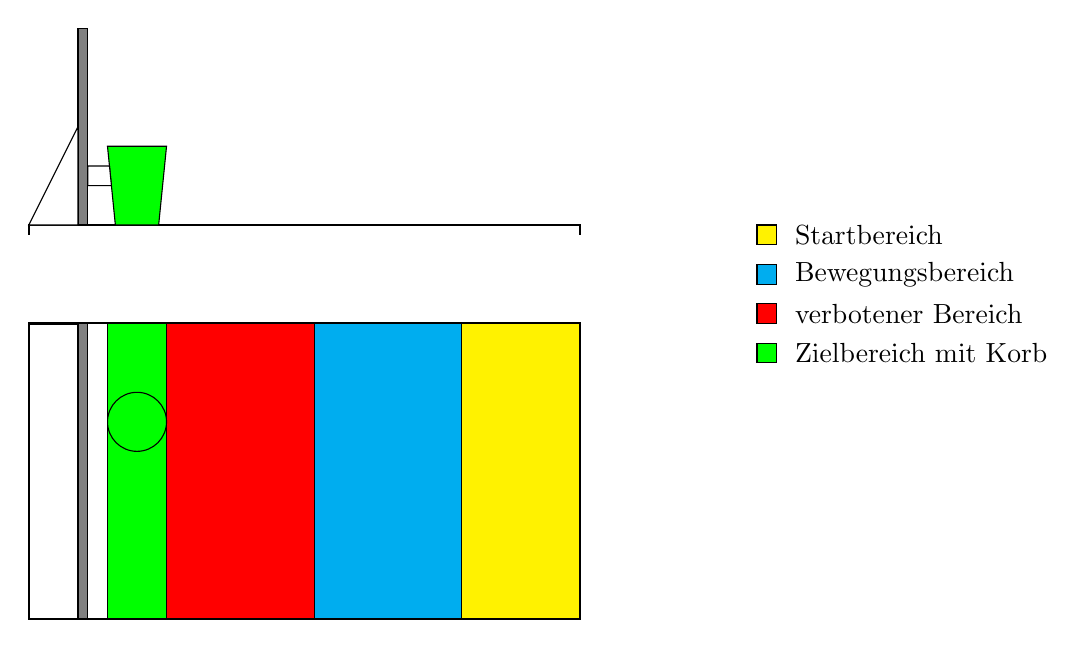
\begin{tikzpicture}[scale=0.025, rotate=90]
        \def \offset {200}          % Offset between Views of playfield
        \def \captionxoffset {130}  % Offset of caption in vertical distance
        \def \captionyoffset {-100} % Offset of caption in horizontal distance
        % playfield frame
        \draw[thick] (0,0) rectangle (150,280);
        \draw[thick] (\offset-5,0) -- (\offset,0) -- (\offset,280) -- (\offset-5,280);
        % startfield
        \draw[fill=yellow] (0,0) rectangle (150,60);
        % move field
        \draw[fill=cyan] (0,60) rectangle (150,135);
        % border line
        \draw[thick] (0,135) -- (150,135);
        % void field
        \draw[fill=red] (0,135) rectangle (150,210);
        % basket field
        \draw[fill=green] (0,210) rectangle (150,240);
        % basket
        \draw[fill=green] (100,225) circle [radius=15];
        \draw[fill=green] (\offset,214) -- (\offset+40,210) -- 
            (\offset+40,240) -- (\offset,236) -- (\offset,214);
        % gap filler
        \draw[fill=white] (0,240) rectangle (150,250);
        \draw[fill=white] (\offset+20,250) -- (\offset+20,238) -- (\offset+30,239) -- (\offset+30,250) -- (\offset+20,250);
        % wall
        \draw[fill=gray] (0,250) rectangle (150,255);
        \draw[fill=gray] (\offset,250) rectangle (\offset+100,255);
        \draw[fill=white] (\offset,255) -- (\offset+50,255) -- (\offset,280) -- (\offset,255);
        % caption
        \draw[fill=green]  (\captionxoffset+00,\captionyoffset) 
            rectangle node[right]{~ Zielbereich mit Korb}   
            (\captionxoffset+10,\captionyoffset+10);
        \draw[fill=red]    (\captionxoffset+20,\captionyoffset) 
            rectangle node[right]{~ verbotener Bereich}     
            (\captionxoffset+30,\captionyoffset+10);
        \draw[fill=cyan]   (\captionxoffset+40,\captionyoffset) 
            rectangle node[right]{~ Bewegungsbereich}       
            (\captionxoffset+50,\captionyoffset+10);
        \draw[fill=yellow] (\captionxoffset+60,\captionyoffset) 
            rectangle node[right]{~ Startbereich}           
            (\captionxoffset+70,\captionyoffset+10);
    \end{tikzpicture}
    \caption{Spielfeld}
    \label{fig:playfield}
\end{figure}


\clearpage
\section{Übersicht Maschinentechnik}

\subsection{Konstruktion mechanische Komponenten}
Die Konstruktion besteht hauptsächlich aus Aluminium-Blechteilen. Einige Komponenten müssen aus konstruktiven Gründen als Frästeile ausgeführt werden. Um ein geringeres Gewicht zu erreichen, werden die Blechteile mit Aussparungen an nicht erforderlichen Flächen versehen. Da dies eine Schwächung der Stabilität mit sich bringt werden die Aussparungen, wie im Flugzeugbau üblich, mit gebogenen Innenkanten ausgeführt.

\begin{figure}[h!]          
	\centering             
	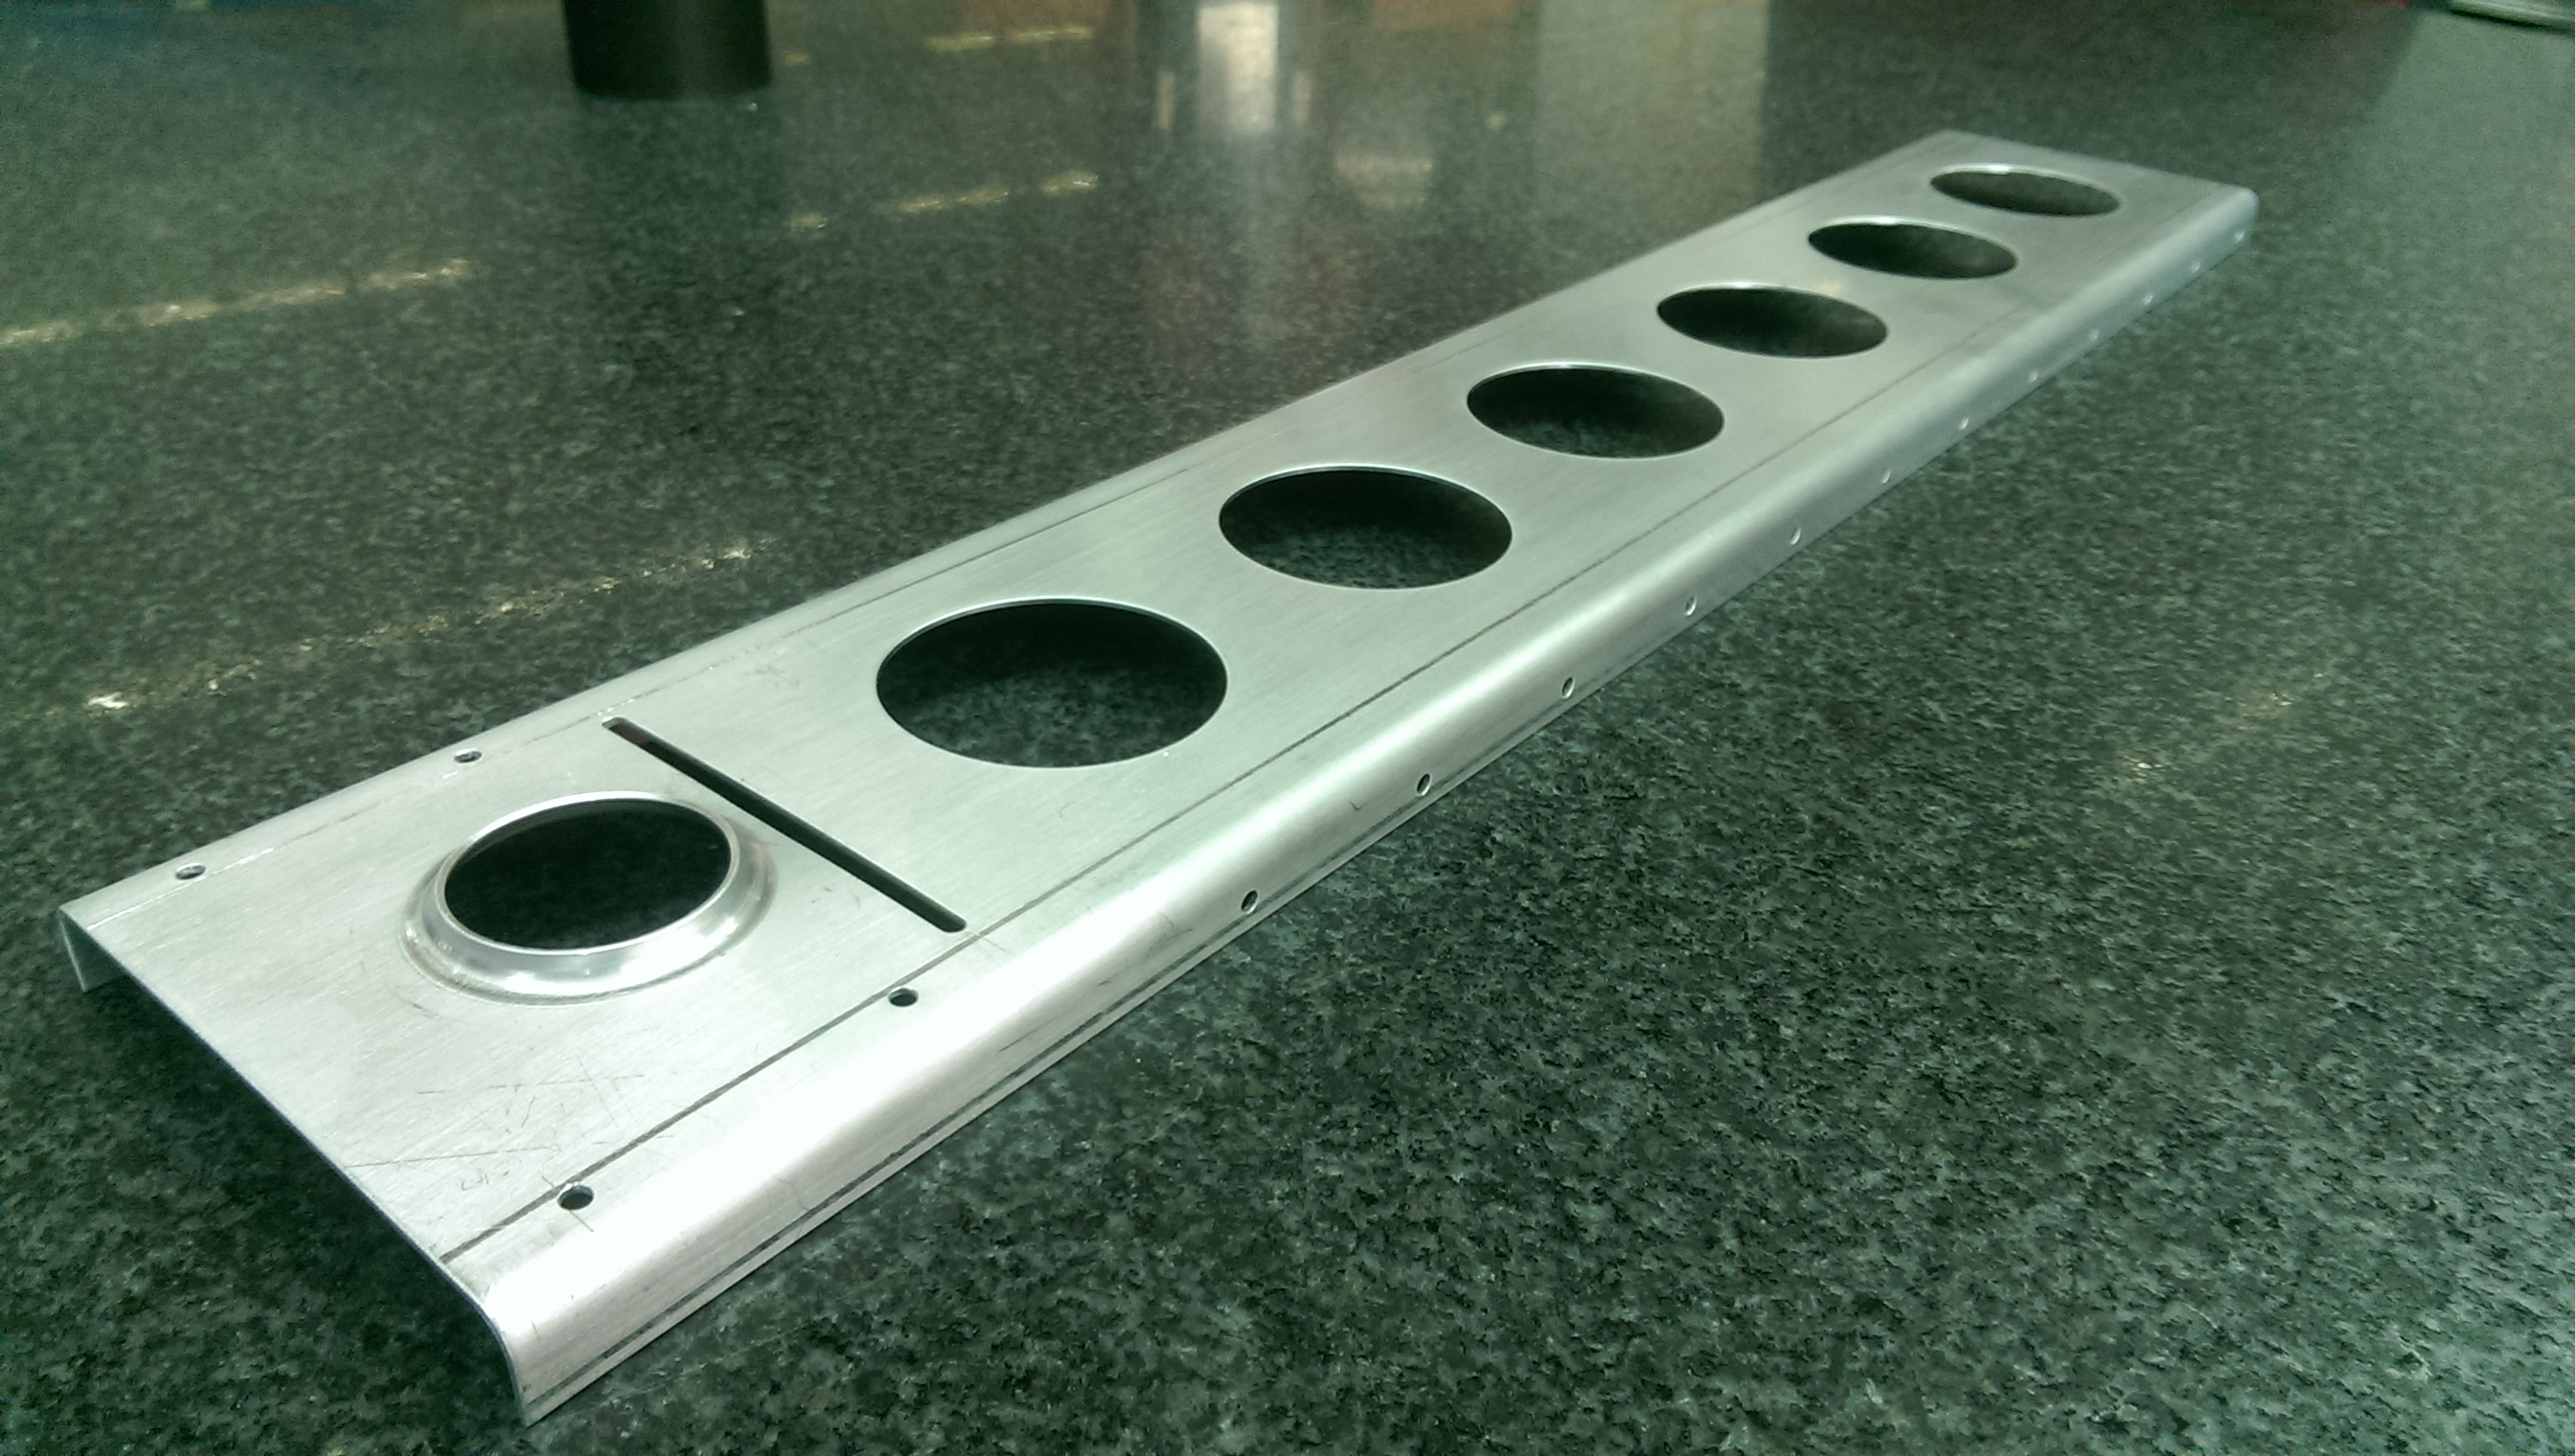
\includegraphics[width=0.5\textwidth]{fig/IMAG0364.jpg}
	\caption{Seitenteil Balllager}
	\label{fig:Seitenteil Balllager}        
\end{figure}

\subsubsection{Ballager}
Das Balllager dient als Grundstruktur, an welcher der Ballnachschub und der 
Motor befestigt sind. Gelagert werden die Bälle im Inneren des quadratischen 
Querschnittes. Die Halterungen des Motors werden jeweils auf beiden 
Aussenseiten des vorderen Endes befestigt. Damit das Stahlband des 
Ballnachschubs optimal aufgewickelt werden kann, werden die herausstehenden 
Enden der Nieten mit Aluminiumleisten abgedeckt.

\subsubsection{Ballnachschub}
Der Ballnachschub besteht im Wesentlichen aus einer Trommel, einem Stahlband 
und einem Servomotor. Das Stahlband wird im Inneren des Balllagers um die 
Bälle herum ausgelegt. Durch das Aufwickeln des Bandes auf die Trommel werden 
die Bälle Richtung Beschleunigungsrad gezogen. Der Antrieb erfolgt durch einen 
umgebauten Servomotor, welcher mittels Zahnriemen mit der Welle der Trommel 
verbunden ist.
\paragraph{Auslegung}
Als Servo dient ein HS85MG der Firma Hitec. Dieses ist wie folgt spezifiziert: 
\begin{table}[h!]
	\centering
	\begin{zebratabular}{lll}
		\rowcolor{gray}
		Parameter &
		Wert bei 4.8\si{\volt} &
		Wert bei 6.0\si{\volt} \\
		Stellgeschwindigkeit (60\si{\degree}) &
		0.16\si{\second} &
		0.14\si{\second} \\
		Drehmoment &
		3.0\si{\kilogram\per\centi\metre} &
		3.5\si{\kilogram\per\centi\metre} \\
	\end{zebratabular}
	\caption{Spezifikation Servomotor}
\end{table}
Dies ergibt folgende Spezifikationen für den sich daraus ergebenden DC Motor: 
\begin{table}[h!]
	\centering
	\begin{zebratabular}{lll}
		\rowcolor{gray}
		Parameter &
		Wert bei 4.8\si{\volt} &
		Wert bei 6.0\si{\volt} \\
		Stellgeschwindigkeit (60\si{\degree}) &
		62.5\si{\per\minute} &
		71.4\si{\per\minute} \\
		Drehmoment &
		0.3\si{\newton\metre} &
		0.35\si{\newton\metre} \\
	\end{zebratabular}
	\caption{Spezifikation DC Motor}
\end{table}

\subsubsection{Drehvorrichtung}
Die Drehvorrichtung dient zur horizontalen Ausrichtung der 
Abschussvorrichtung. Um eine genaue Positionierung und ausreichende Stabilität 
zu ermöglichen, wurde ein Zahnrad durch zwei Axial-Rillenkugellager auf einer 
Grundplatte verspannt. Die Ausrichtung wird durch einen Schrittmotor mit dem 
direkt verbundenen, kleineren Zahnrad eingestellt. Einen guten Bodenkontakt 
garantieren an der Unterseite der Füsse angeklebte Gummimatten.

\paragraph{Auflösung}
Der Schrittmotor benötigt 200 Schritte für eine Umdrehung. Er wird mit 1/128 
Mikrosteps angesteuert. Die Übersetzung beträgt 1:4.8. Daraus ergibt sich 
folgende Auflösung: 
\[ 200 \cdot 128 \cdot 4.8 = 122'880 \frac{\text{Schritte}}{\text{Umdrehung}}  \]
\[ \frac{360^\circ}{122'880} = 0.0029296875 \frac{^\circ}{\text{Schritt}} 
= 0.17578 \frac{'}{\text{Schritt}} = 10.547 \frac{''}{\text{Schritt}}
\rightarrow 341.33 \frac{\text{Schritte}}{^\circ}\]

\subsubsection{Motor}
Der Motor wird als Eigenkonstruktion ausgeführt. Der Läufer wird auf einer 
CNC-Fräsmaschine gefräst, wobei dieser sogleich als Felge des 
Beschleunigungsrades dient. Aufgrund der magnetischen Eigenschaften muss 
zusätzlich ein Stahlring eingepresst werden. Als Grundlage für den Stator 
dienen Statorbleche von Motoren aus Diskettenlaufwerken. Aus diesen wird ein 
neuer Stator mit doppelter Dicke erstellt. Dieser wird anschliessend neu 
bewickelt. 

\subsubsection{Turm}
Der Turm dient als Verbindungselement des Balllagers mit dem grösseren Zahnrad 
der Drehvorrichtung. Ausgeführt wird die gesamte Konstruktion aus 
Aluminiumblech. Der Platz im Inneren wird zum Verstauen der 
Elektronikkomponenten verwendet. Hierfür wird die vordere Abdeckplatte statt 
mit Nieten, mit Schrauben befestigt.

\clearpage
\subsection{Herstellung mechanische Komponenten}
Die konzeptionellen CAD-Zeichnungen werden ab Semesterwoche 2 weiter 
ausgearbeitet, abgewickelt und die Fertigungszeichnungen erstellt. Hierbei 
müssen hauptsächlich Details wie Bohrungen für die Nieten angebracht und 
einige konstruktive Anpassungen vorgenommen werden. 

Ab Semesterwoche 3 können die ersten Teile an der Fräsmaschine im 
Elektrotechniklabor produziert werden, wobei parallel  hierzu die restlichen 
Komponenten am CAD fertiggestellt werden.  Um die gebogenen Innenkanten der 
Aussparungen zu realisieren, werden die gefrästen Blechteile mit einer 
Handpresse und eigens hierfür hergestellten Werkzeugen gefertigt.

In Semesterwoche 4 werden die Grundplatte zur Fertigung an der HSLU in Auftrag 
gegeben.

In Semesterwoche 5 werden zusätzlich einige Teile zum spanenden Herstellen, 
sowie zum 3D-Drucken in Auftrag gegeben. Ebenfalls wird eine 
Rohmaterialbestellung abgegeben.

Die in Auftrag gegebenen Teile können in Semesterwoche 6 abgeholt werden, 
wobei das  Rohmaterial fälschlicherweise aus Stahl, anstatt aus Aluminium, 
bestellt wurde. Eine neue Bestellung des richtigen Rohmaterials wurde abgesetzt.

In Semesterwoche 7 können die bestellten Teile sowie die zum biegen extern in 
Auftrag gegebenen Teile abgeholt werden. Des weiteren wird mit dem Zusammenbau 
der einzelnen Komponenten begonnen. Aufgrund eines beim Biegen entstandenen 
Verzugs einzelner Bauteile und einiger konstruktiver Ungenauigkeiten müssen 
diverse Bohrungen durch feilen nachgebessert werden. Durch Niethefter kann die 
Konstruktion bis zum endgültigen Vernieten aufgebaut werden.

\begin{figure}[h!]          
	\centering             
	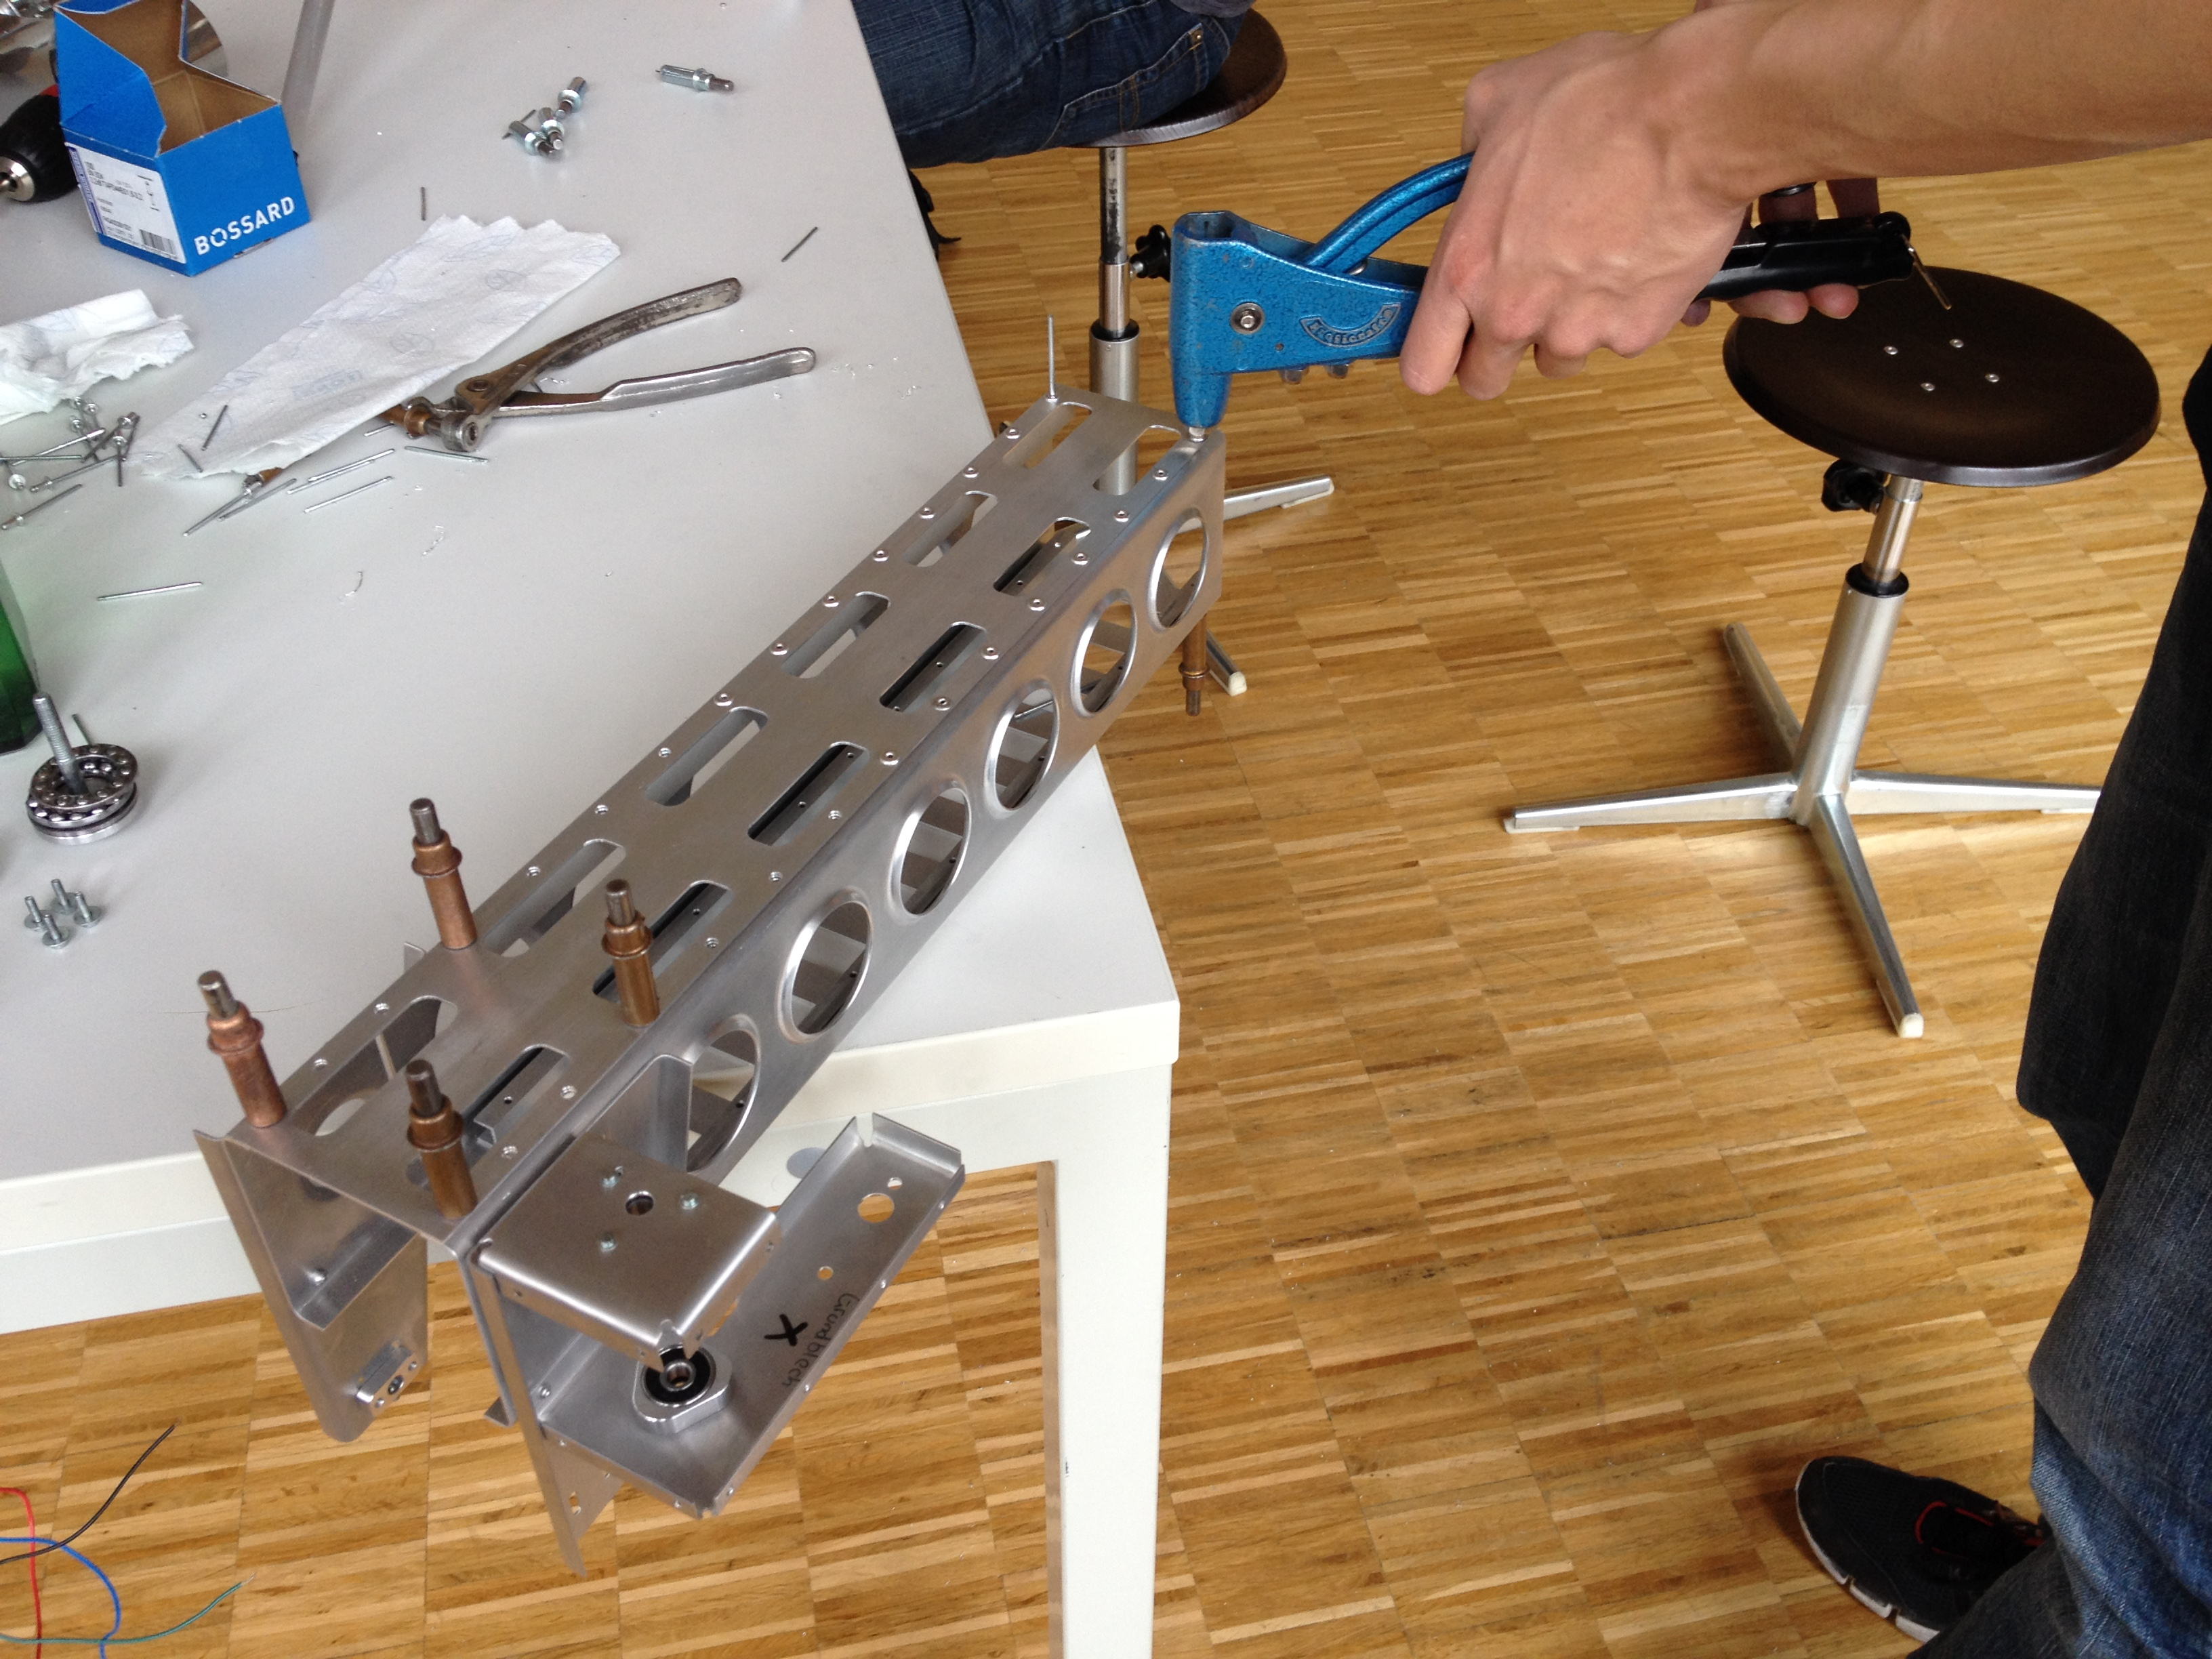
\includegraphics[width=0.5\textwidth]{fig/IMG_2290.JPG}
	\caption{Zusammenbau Balllager}
	\label{fig:Zusammenbau Balllager}        
\end{figure}

\begin{figure}[h!]          
	\centering             
	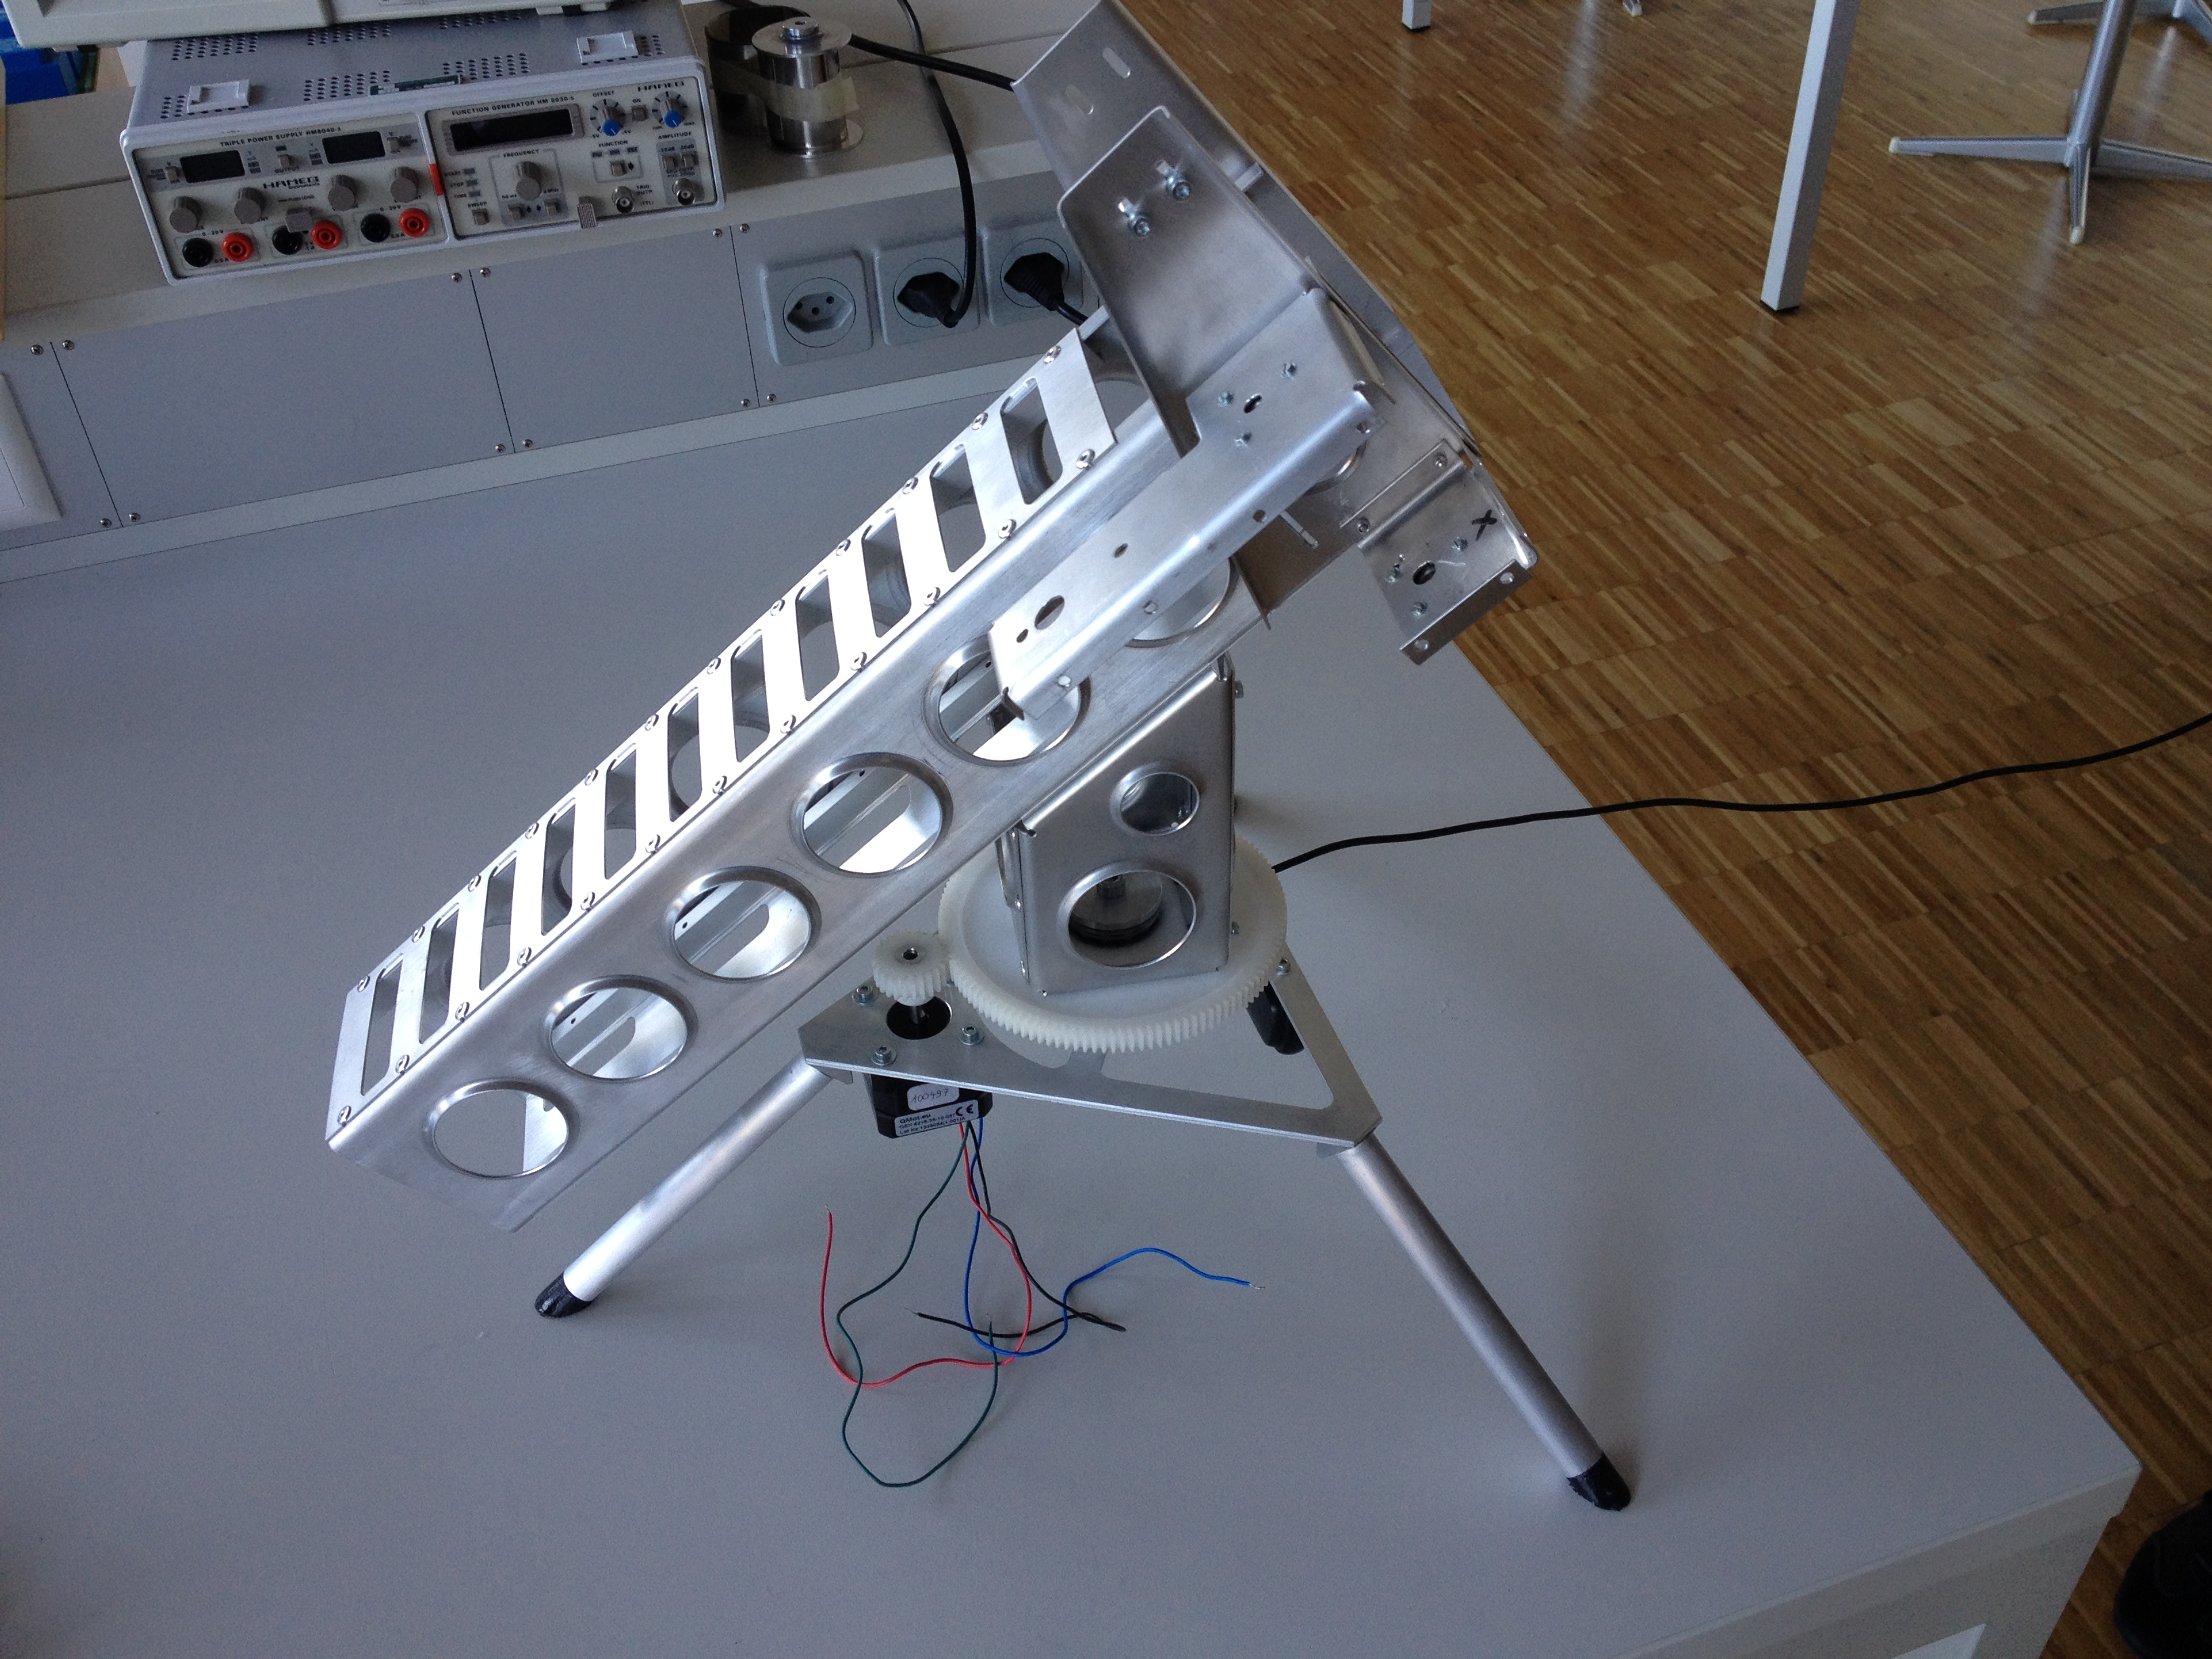
\includegraphics[width=0.5\textwidth]{fig/IMG_2303.JPG}
	\caption{Unvollständiger Aufbau}
	\label{fig:Unvollständiger Aufbau}        
\end{figure}

\subsubsection{Balllager}
Anhand der Erfahrungen erster Testläufe wird entschieden, keine Verstärkung an 
der Unterseite des vorderen Endes anzubringen. Diese Verstärkung hätte eine zu 
starke Durchbiegung des Blechs beim Abschuss der Bälle verhindert.

\subsubsection{Ballnachschub}
Beim Zusammenbau wird festgestellt, dass die Welle der Trommel einen zu 
grossen Durchmesser hat und daher mit Hilfe einer Handbohrmaschine und 
gewöhnlichem Schleifpapier auf das gewünschte Mass geschliffen werden muss.

\subsubsection{Drehvorrichtung}
Um weiteres Gewicht einzusparen wird die bereits hergestellte Grundplatte auf 
die halbe Höhe überfräst.

\begin{figure}[h!]          
	\centering             
	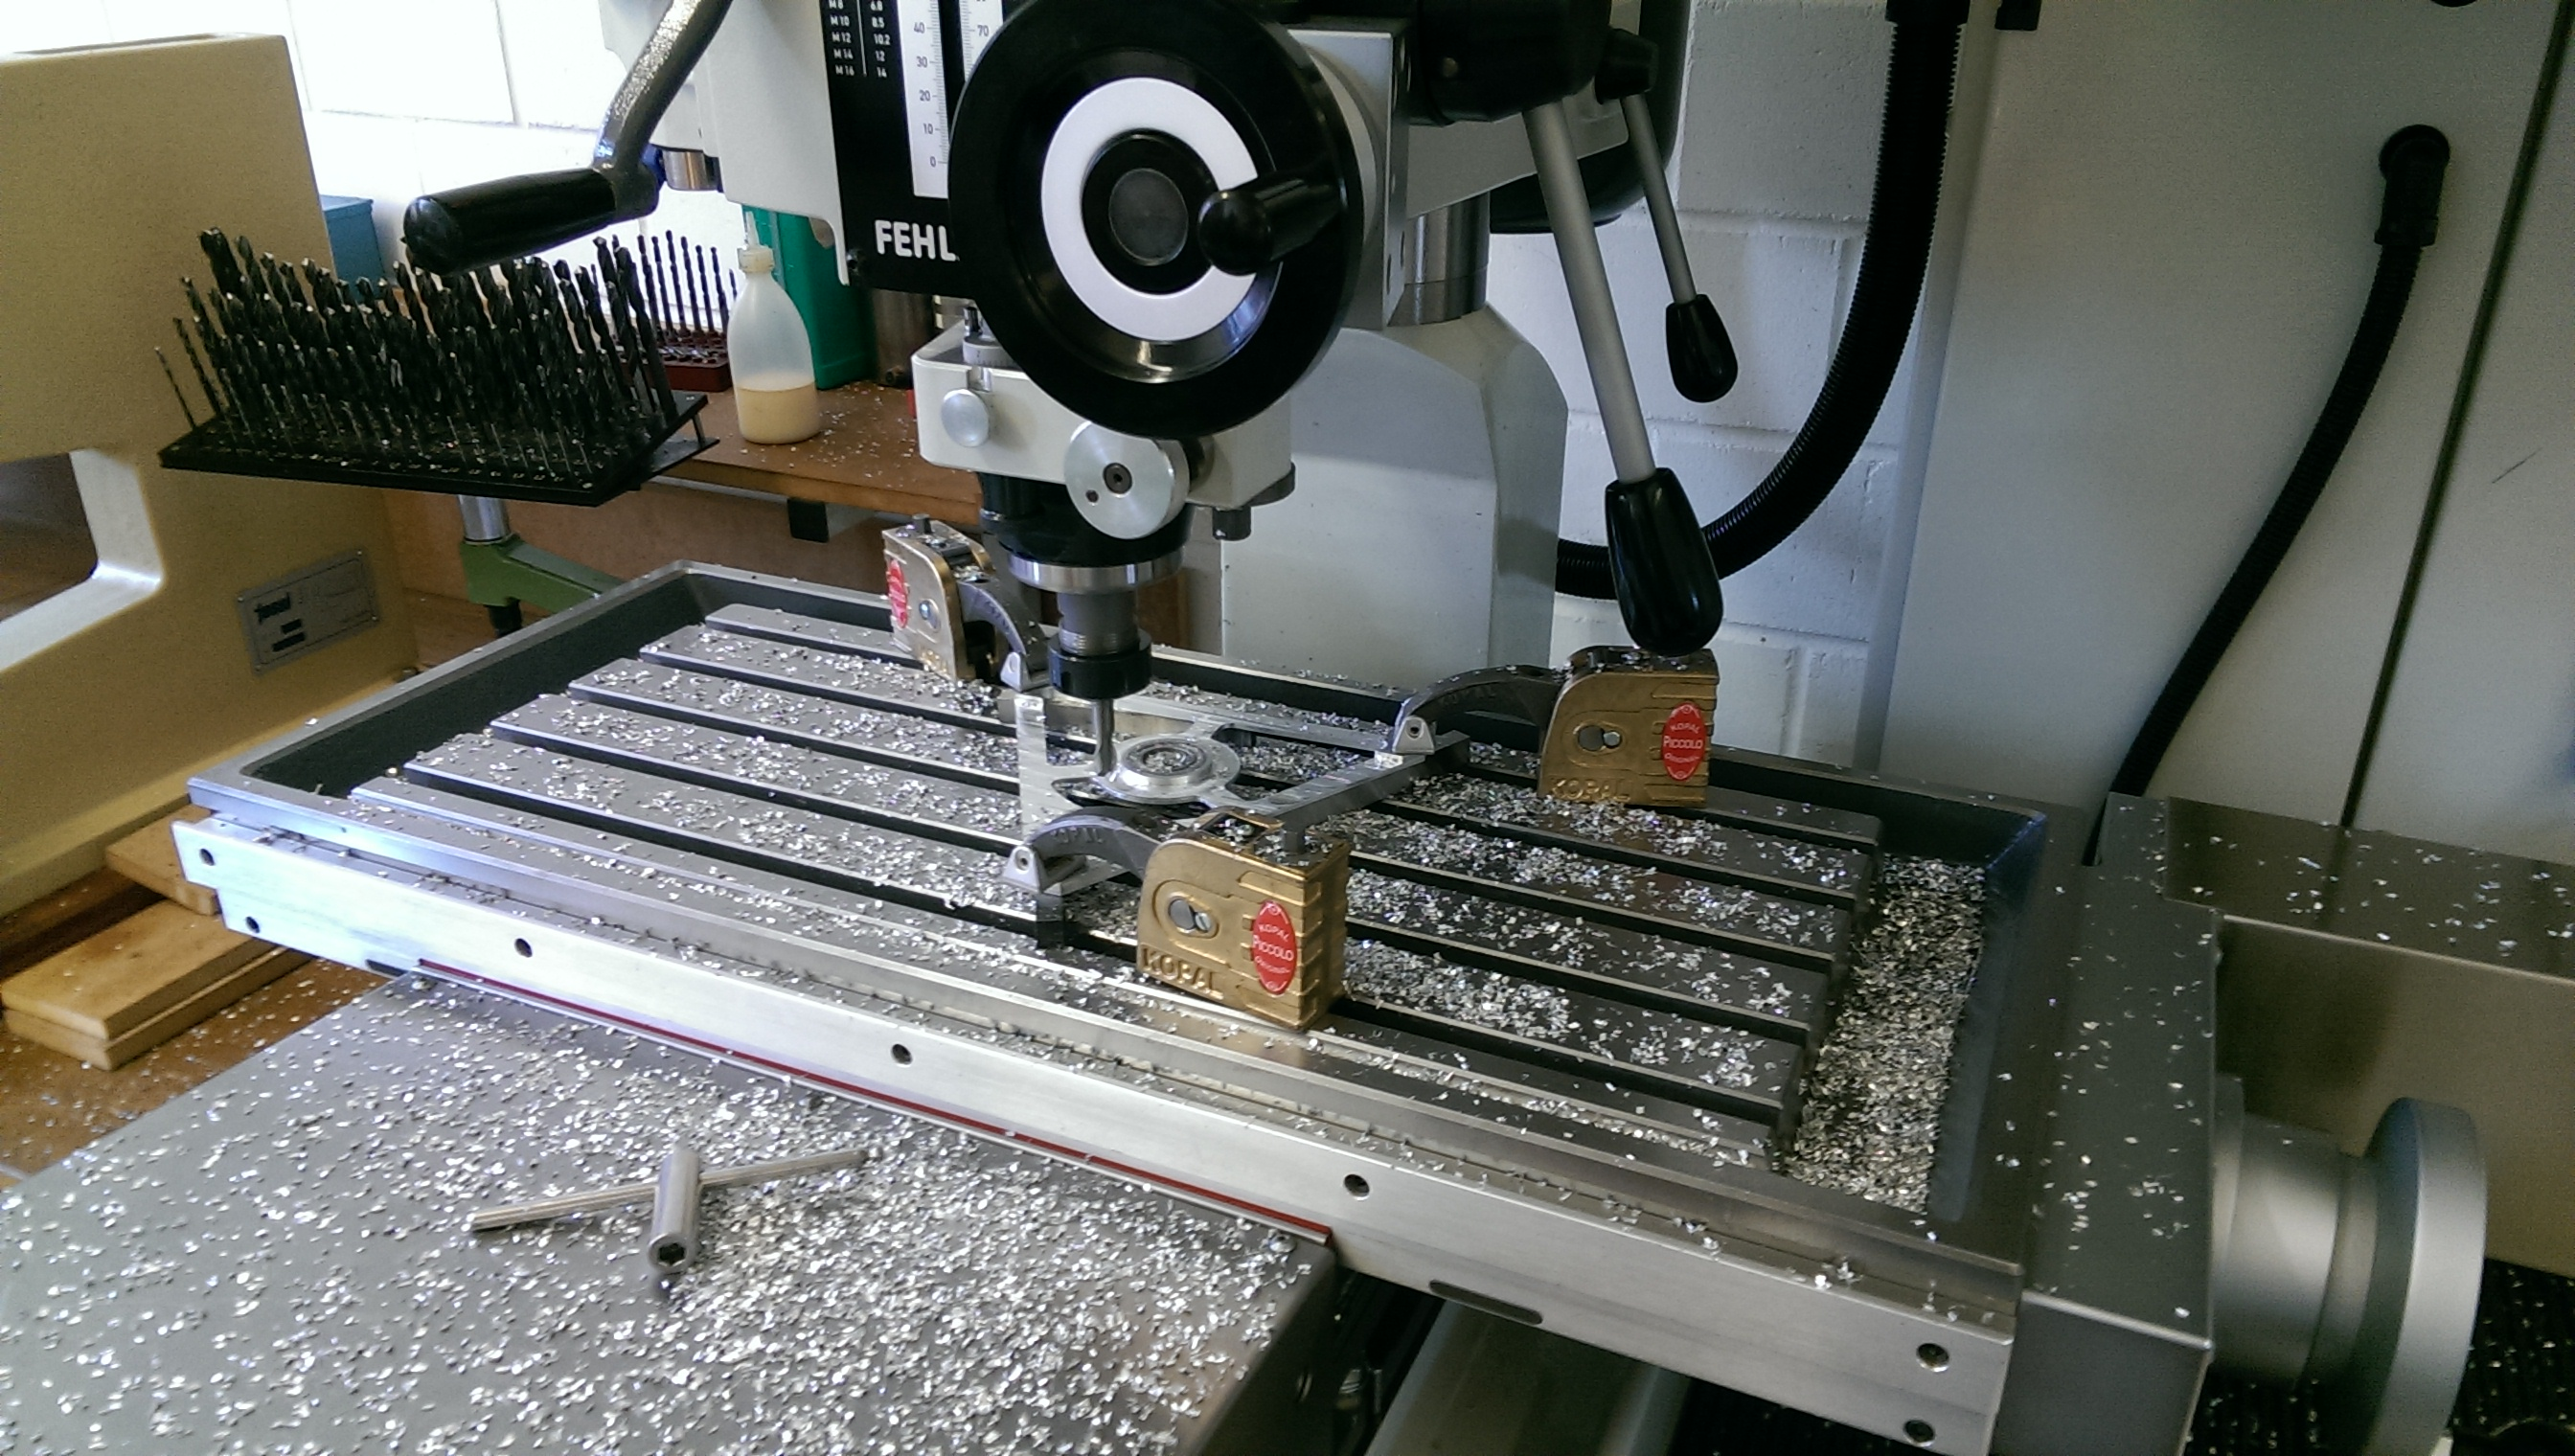
\includegraphics[width=0.5\textwidth]{fig/IMAG0357.jpg}
	\caption{Überfräsen der Grundplatte}
	\label{fig:Grundplatte fräsen}        
\end{figure}

\subsubsection{Motor}
Sämtliche Magnete werden von Hand eingesetzt und mit Zweikomponentenklebstoff 
befestigt. Der Stator wird aus gebrauchten Floppydisk-Laufwerken ausgebaut, 
neu gewickelt und an einer gefrästen Halterung befestigt.

Beim Zusammenbau wird bemerkt, dass die Langlöcher der Motorenhalterung zu 
kurz ausgeführt wurden um einen guten Anpressdruck der Bälle zu ermöglichen. 
Daher werden diese durch feilen verlängert.

\subsubsection{Turm}
Die Muttern werden auf der Innenseite des Turms mit Zweikomponentenklebstoff 
angebracht.

\begin{figure}[h!]          
	\centering             
	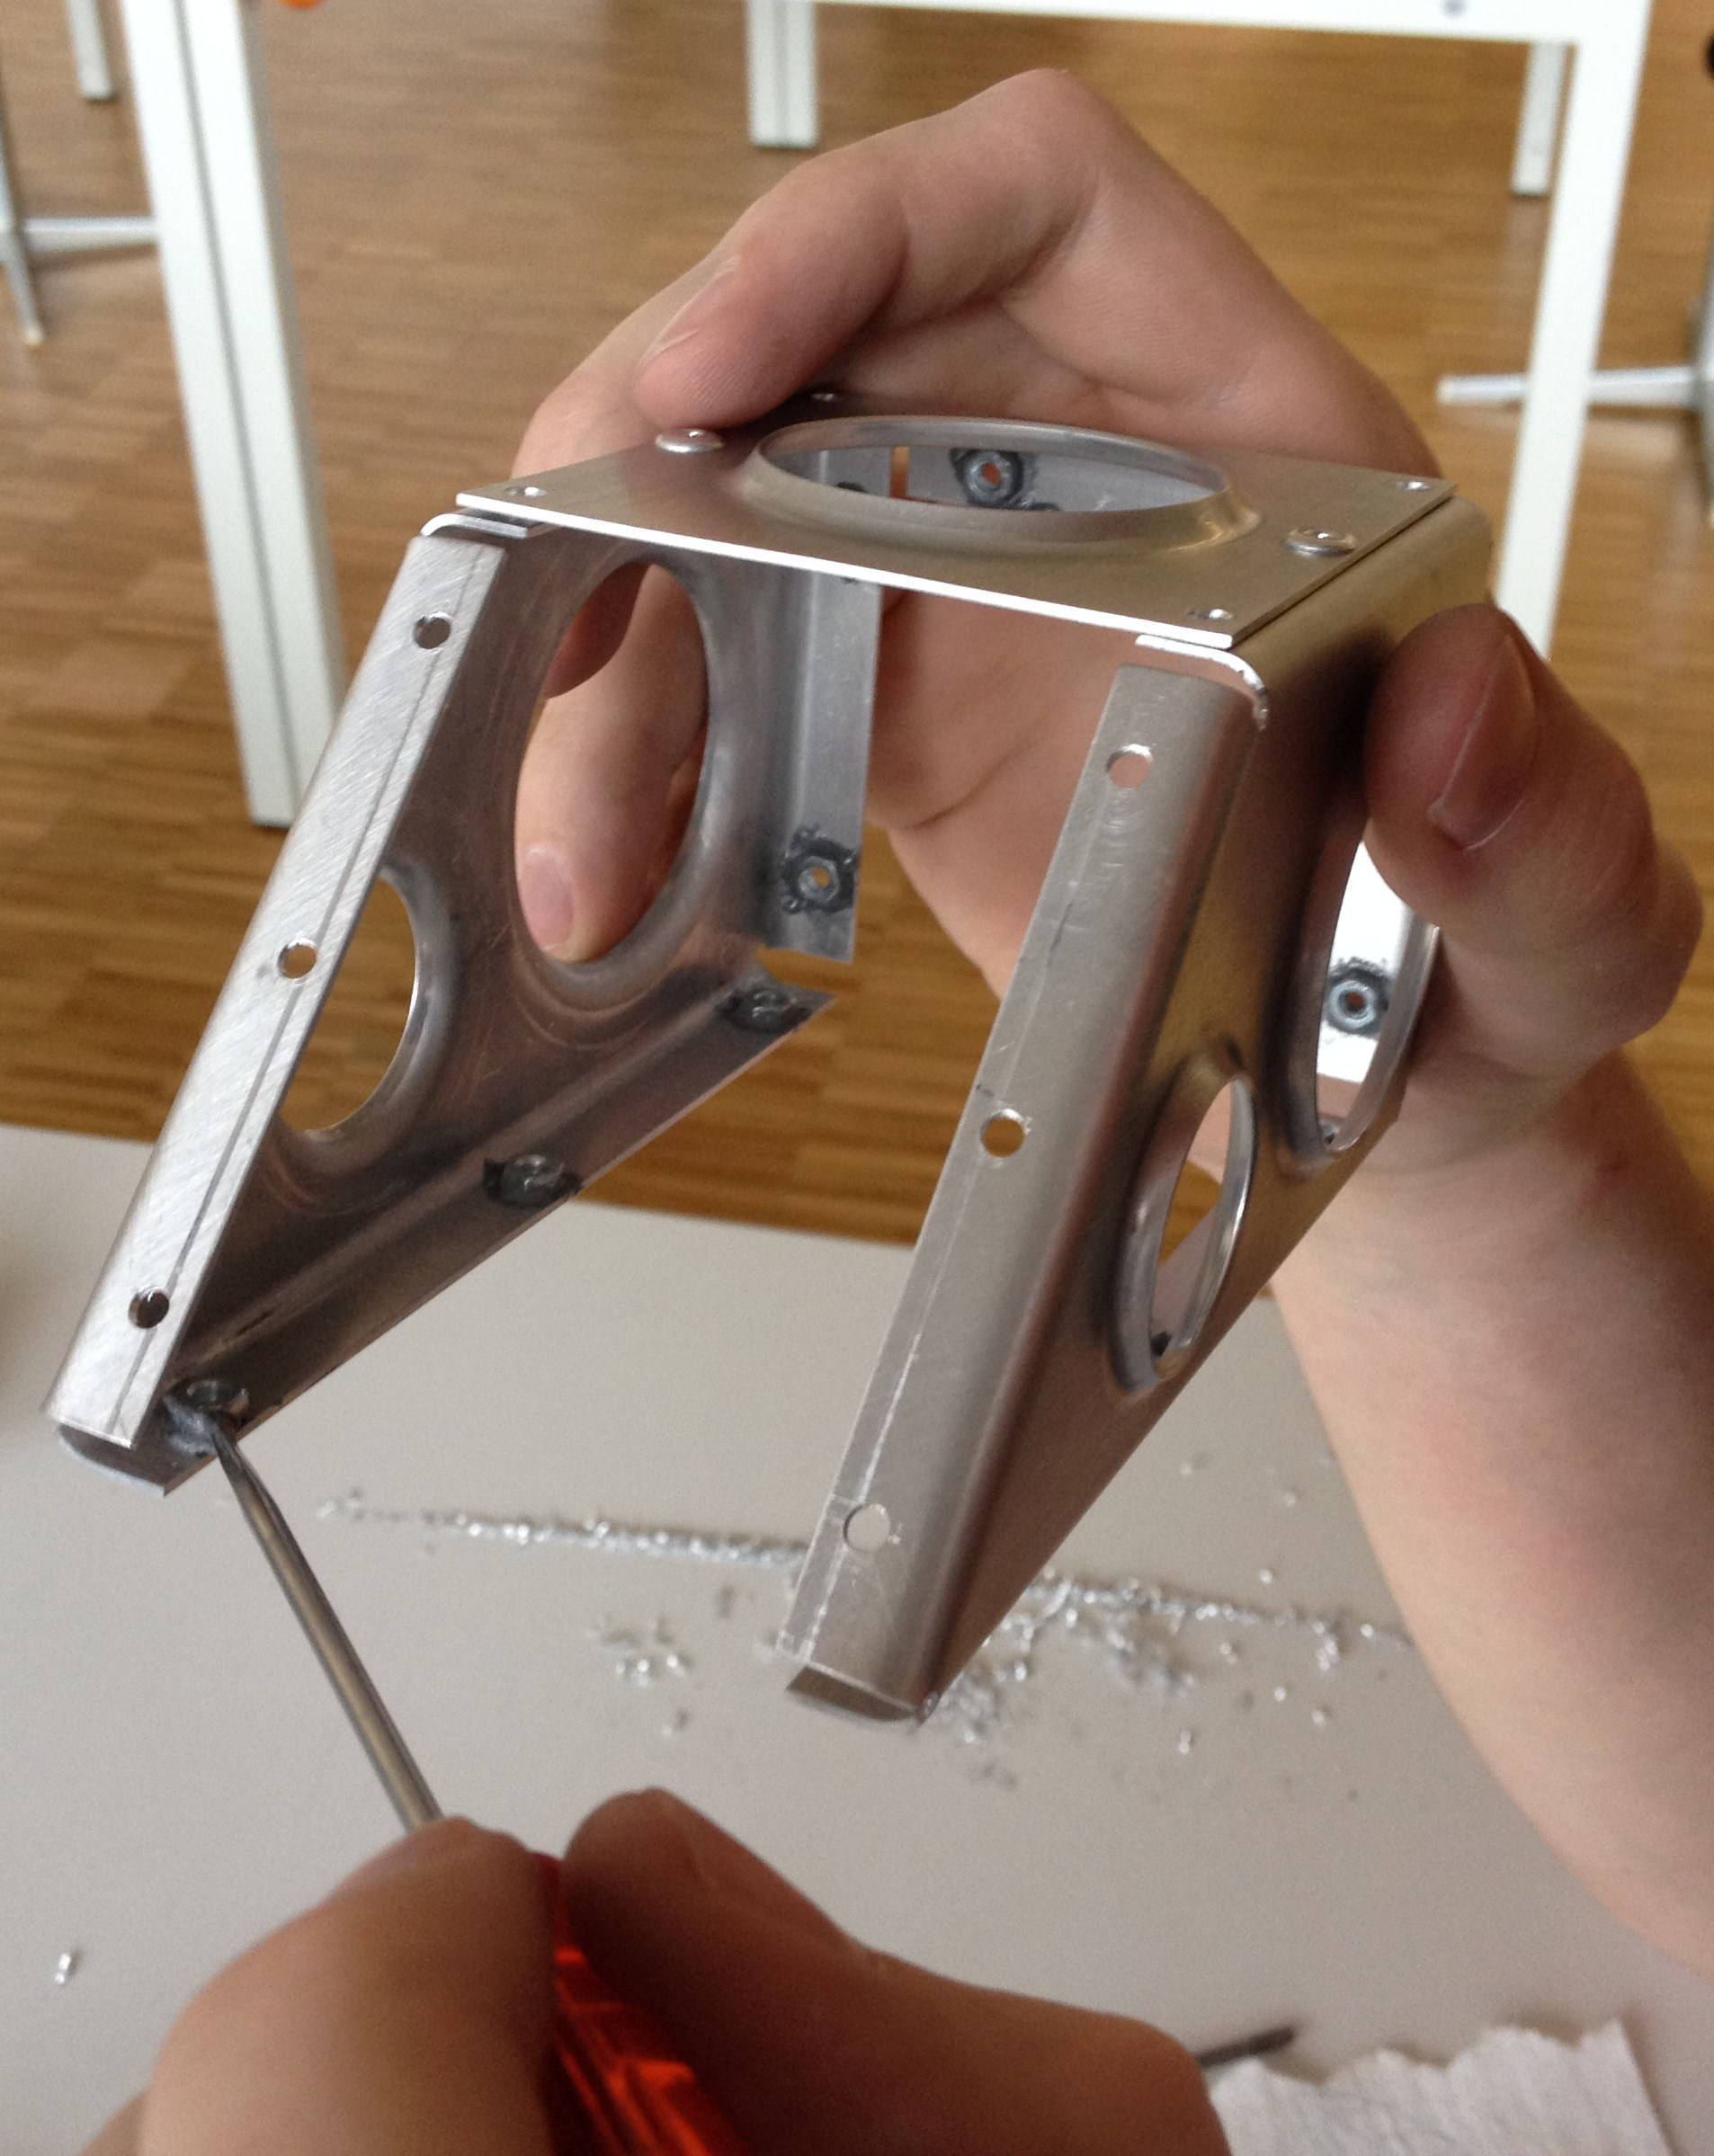
\includegraphics[width=0.3\textwidth]{fig/IMG_2292.JPG}
	\caption{Kleben der Muttern}
	\label{fig:Muttern Kleben}        
\end{figure}



\clearpage
\subsection{Balllager}
Das Balllager dient als Grundstruktur, auf welcher der Ballnachschub und der Motor befestigt sind. Gelagert werden die Bälle im Inneren des quadratischen Querschnittes. Die Halterungen des Motors wird jeweils auf 
beiden Aussenseiten des vorderen Endes befestigt. Damit das Stahlband des Ballnachschubs optimal aufgewickelt werden kann, werden die herausstehenden Enden der Nieten mit Aluminiumleisten abgedeckt.

Anhand der Erfahrungen erster Testläufe wird entschieden, keine Verstärkung an der Unterseite des Vorderen Endes anzubringen. Diese Verstärkung hätte eine zu starke Durchbiegung des Blechs beim Abschuss der Bälle verhindert.

\clearpage
\subsection{Ballnachschub}
Der Ballnachschub besteht aus einer Halterung, Trommel, Stahlband und einem Servomotor. Das Stahlband wird im Inneren des Balllagers um die Bälle herum ausgelegt. Durch das Aufwickeln des Bandes auf die Trommel werden die Bälle Richtung Beschleunigungsrad gezogen. Der Antrieb erfolgt durch einen 
umgebauten Servomotor, welcher mittels Zahnriemen mit der Welle der Trommel verbunden ist.

Beim Zusammenbau wird festgestellt, dass die Welle der Trommel einen zu grossen Durchmesser hat und daher von Hand auf das gewünschte Mass geschliffen werden muss.

\subsubsection{Auslegung}
Als Servo dient ein HS85MG der Firma Hitec. Dieses ist wie folgt spezifiziert: 
\begin{table}[h!]
    \centering
    \begin{zebratabular}{lll}
        \rowcolor{gray}
        Parameter &
            Wert bei 4.8\si{\volt} &
            Wert bei 6.0\si{\volt} \\
        Stellgeschwindigkeit (60\si{\degree}) &
            0.16\si{\second} &
            0.14\si{\second} \\
        Drehmoment &
            3.0\si{\kilogram\per\centi\metre} &
            3.5\si{\kilogram\per\centi\metre} \\
    \end{zebratabular}
    \caption{Spezifikation Servomotor}
\end{table}
Dies ergibt folgende Spezifikationen für den sich daraus ergebenden DC Motor: 
\begin{table}[h!]
    \centering
    \begin{zebratabular}{lll}
        \rowcolor{gray}
        Parameter &
            Wert bei 4.8\si{\volt} &
            Wert bei 6.0\si{\volt} \\
        Stellgeschwindigkeit (60\si{\degree}) &
            62.5\si{\per\minute} &
            71.4\si{\per\minute} \\
        Drehmoment &
            0.3\si{\newton\metre} &
            0.35\si{\newton\metre} \\
    \end{zebratabular}
    \caption{Spezifikation DC Motor}
\end{table}


\clearpage
\subsection{Drehvorrichtung}
Die Drehvorrichtung dient zur horizontalen Ausrichtung der 
Abschussvorrichtung. Um eine genaue Positionierung und ausreichende Stabilität 
zu ermöglichen, wurde ein Zahnrad mit dem Durchmesser igjdsjs durch zwei 
Axial-Rillenkugellager auf einer Grundplatte verspannt. Die Ausrichtung wird 
durch einen Schrittmotor mit dem direkt verbundenen, kleineren Zahnrad 
eingestellt. Einen guten Bodenkontakt garantieren drei, an der Grundplatte 
befestigte Beine.

\subsubsection{Auflösung}
Der Schrittmotor benötigt 200 Schritte für eine Umdrehung. Er wird mit 1/128 
Mikrosteps angesteuert. Die Übersetzung beträgt 1:4.8. Daraus ergibt sich 
folgende Auflösung: 
\[ 200 \cdot 128 \cdot 4.8 = 122'880 \frac{\text{Schritte}}{\text{Umdrehung}}  \]
\[ \frac{360^\circ}{122'880} = 0.0029296875 \frac{^\circ}{\text{Schritt}} 
= 0.17578 \frac{'}{\text{Schritt}} = 10.547 \frac{''}{\text{Schritt}}
\rightarrow 341.33 \frac{\text{Schritte}}{^\circ}\]

\clearpage
\section{Motor}
Der Motor wurde als Eigenkonstruktion ausgeführt. Der Läufer wurde auf einer 
CNC-Fräsmaschine gefräst, wobei dieser sogleich als Felge des 
Beschleunigungsrades fungiert. Aufgrund der magnetischen Eigenschaften musste 
zusätzlich ein Stahlring eingepresst werden. Auch wurden sämtliche Magnete von 
Hand eingesetzt. Der fguiwehn wurde aus gebrauchten Floppydisk-Lauferken 
ausgebaut, neu gewickelt und an einer Halterung befestigt.

\clearpage
\subsection{Turm}
Der Turm dient als Verbindungselement des Balllager und des grösseren 
Zahnrades der Drehvorrichtung. Ausgeführt wurde die gesamte Konstruktion aus 
Aluminiumblech. Der Platz im Inneren wird zum Verstauen der 
Elektronikkomponenten verwendet.

\clearpage
\section{Übersicht Elektronik}
\tikzstyle{block} = [ rectangle, rounded corners, minimum width=1.5cm, minimum height=1cm, draw=black ]
\begin{figure}[h!]
    \centering
    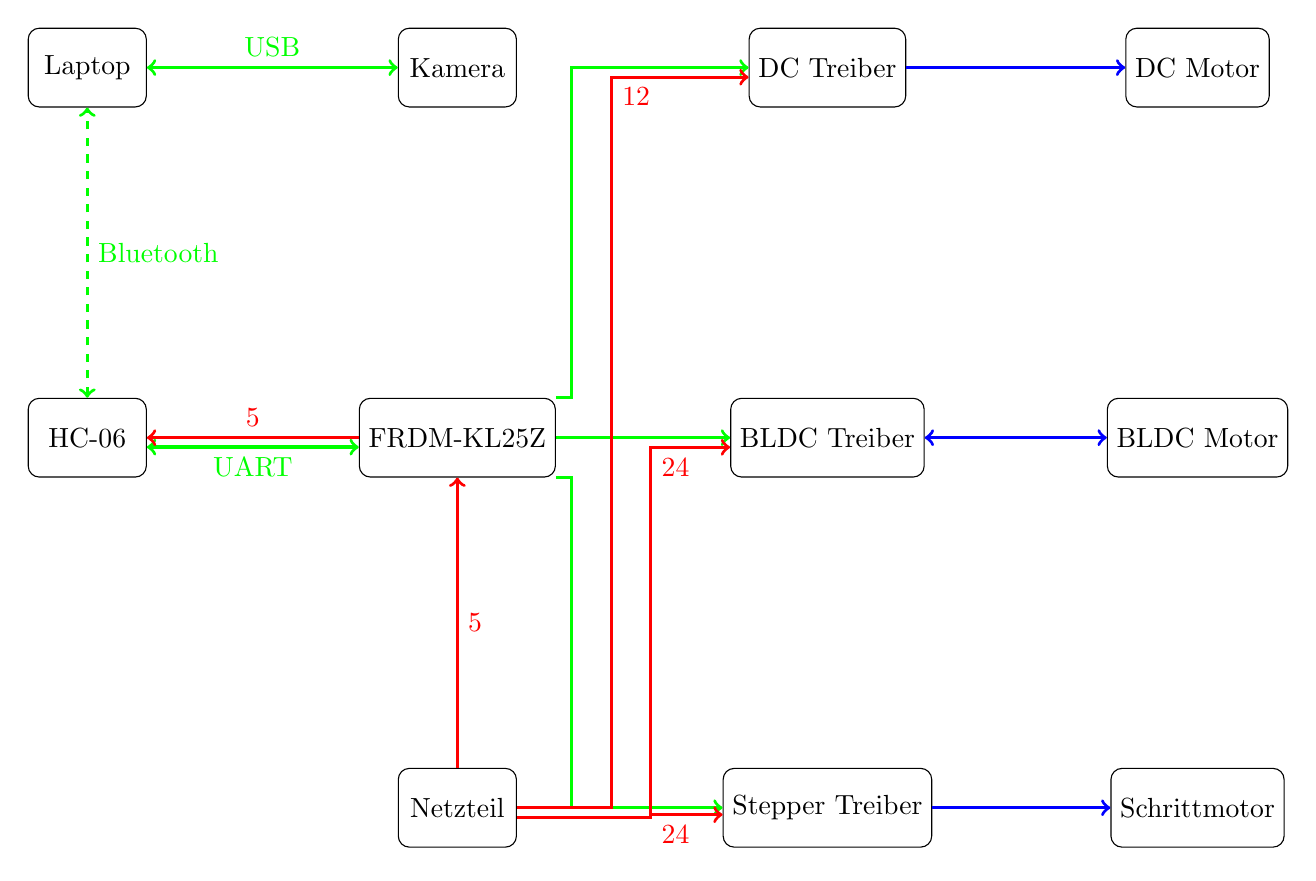
\begin{tikzpicture}[node distance=4.7cm]
        \node (frdm)        [block]                     {FRDM-KL25Z};
        \node (bt)          [block, left  of=frdm]      {HC-06};
        \node (computer)    [block, above of=bt]        {Laptop};
        \node (camera)      [block, right of=computer]  {Kamera};
        \node (supply)      [block, below of=frdm]      {Netzteil};
        \node (bldc-drv)    [block, right of=frdm]      {BLDC Treiber};
        \node (bldc)        [block, right of=bldc-drv]  {BLDC Motor};
        \node (step-drv)    [block, below of=bldc-drv]  {Stepper Treiber};
        \node (step)        [block, right of=step-drv]  {Schrittmotor};
        \node (dc-drv)      [block, above of=bldc-drv]  {DC Treiber};
        \node (dc)          [block, right of=dc-drv]    {DC Motor};
        % Data connections
        \draw[very thick, ->, green]    (frdm.south east)   -| ++(0.2cm, 0)     |- (step-drv.west);
        \draw[very thick, ->, green]    (frdm.east)         -| ++(0.2cm, 0)     |- (bldc-drv.west);
        \draw[very thick, ->, green]    (frdm.north east)   -| ++(0.2cm, 0)     |- (dc-drv.west);
        \draw[very thick, <->, green]   (frdm.base west)    -- node[below] {UART} (bt.base east);
        % Wireless data connection
        \draw[very thick, <->, green, dashed]   (bt)        -- node[right] {Bluetooth} (computer);
        \draw[very thick, <->, green]           (camera)    -- node[above] {USB} (computer);
        % Motor Power connections
        \draw[very thick, ->, blue]     (step-drv)  -- (step);
        \draw[very thick, <->, blue]    (bldc-drv)  -- (bldc);
        \draw[very thick, ->, blue]     (dc-drv)    -- (dc);
        % Power connections
        \draw[very thick, ->, red]  (frdm.west)         -- node[above] {5\si{\volt}}    (bt.east);
        \draw[very thick, ->, red]  (supply.north)      -- node[right] {5\si{\volt}}    (frdm);
        \draw[very thick, ->, red]  (supply.base east) -| ++(1.7cm, 0)     |- node[below right] {24\si{\volt}} (step-drv.base west);
        \draw[very thick, ->, red]  (supply.base east) -| ++(1.7cm, 0)     |- node[below right] {24\si{\volt}} (bldc-drv.base west);
        \draw[very thick, ->, red]  (supply.east) -| ++(1.2cm, 0)     |- node[below right] {12\si{\volt}} (dc-drv.base west);
    \end{tikzpicture}
    \caption{Übersicht Elektrotechnik}
\end{figure}

\clearpage
\subsection{Fachgruppe Elektrotechnik}
\label{sec:pren-et}
Elektrotechnik-Studierende aus mehreren Gruppen haben sich
zusammengeschlossen, um gemeinsame Probleme anzugehen. Dabei handelt es sich
um die benötigte Hard- und Software, um Motoren anzusteuern
und gegebenenfalls zu regeln. In diesem Zusammenschluss werden drei Gruppen
gebildet, um Lösungen für DC-, Stepper- und Brushless-Motoren auszuarbeiten.
Die Idee besteht darin, dass nicht jede Gruppe für dasselbe Problem womöglich 
denselben Lösungsansatz verfolgt, sondern die Ressourcen kombiniert,
Synergien nutzt, um eine bessere Lösung zu erarbeiten. Auf diese Weise kann
das teamübergreifende Arbeiten im Rahmen des PREN erlernt und
geübt werden. Somit wird Idee der Interdisziplinarität im erweiterten Sinn
Rechnung getragen. Die Gruppen und deren Mitglieder sind in 
\autoref{tab:pren-et-members} aufgeführt.
\begin{table}[h!]
    \centering
    \begin{zebratabular}{lllccc}
        \rowcolor{gray} 
        Team & Mitglied         & Github    & DC          & BLDC        & Stepper     \\
        27   & Daniel Winz      & daniw     &             & \textbullet & \textbullet \\
        32   & Yves Studer      & ystuder   &             & \textbullet &             \\
        33   & Flavio Kreiliger & Flavinsky & \textbullet &             & \textbullet \\
        38   & Bettina Wyss     & BettyET   &             &             & \textbullet \\
        39   & Ervin Mazlagi\'c & ninux     & \textbullet &             &             \\
    \end{zebratabular}
    \caption{Übersicht der PREN-ET Projektgruppen}
    \label{tab:pren-et-members}
\end{table}
Für den Austausch und die Ablage von Daten und Unterlagen wird die Plattform 
Github ausgewählt, da damit via Git\footnote{Verteiltes 
Versionskontrollsystem} versioniert werden kann. Dazu wird auf Github die 
Organisation PREN-ET gegründet. Diese ist unter 
\url{https://github.com/PREN-ET} einsehbar. für die einzelnen Projekte werden 
Repositories angelegt. Diese sind in \autoref{tab:pren-et-repos} aufgeführt. 
\begin{table}[h!]
    \centering
    \begin{zebratabular}{p{0.09\textwidth}p{0.37\textwidth}p{0.4\textwidth}}
        \rowcolor{gray} 
        Repository  & Link         & Beschreibung \\
        info        & \url{https://github.com/PREN-ET/info}    & Allgemeine Informationen zur Organisation von PREN-ET \\
        doc         & \url{https://github.com/PREN-ET/doc}     & Dokumentation \\
        dc          & \url{https://github.com/PREN-ET/dc}      & Treiber für Gleichstrommotoren \\
        bldc        & \url{https://github.com/PREN-ET/bldc}    & Treiber für Brushless Motoren \\
        stepper     & \url{https://github.com/PREN-ET/stepper} & Treiber für Schrittmotoren \\
        frdm        & \url{https://github.com/PREN-ET/frdm}    & Beispiele zur Ansteuerung mittels FRDM-KL25Z \\
    \end{zebratabular}
    \caption{Übersicht der PREN-ET Repositories}
    \label{tab:pren-et-repos}
\end{table}

\clearpage
\subsection{Energieversorgung}
Der Schrittmotor und der BLDC Motor werden mit einer Spannung von 48\si{\volt} 
betrieben. Der DC Motor für die Ballnachführung und die Kontrollplatine werden 
mit einer Spannung von 5\si{\volt} versorgt. Dazu werden Netzteile aus Servern 
verwendet. Davon werden vier in Serie geschaltet um die notwendige Spannung 
von 48\si{\volt} zu erreichen. Um Kurzschlüsse zu vermeiden, müssen die 
Netzteile potentialfrei gemacht werden. Bei den verwendeten Netzteilen vom Typ 
PS-3701-1 von HP wird die Sekundärseite mit einer Schraube elektrisch mit dem 
Gehäuse verbunden. Das Gehäuse ist mit PE verbunden und somit geerdet. Diese 
Schraube wird durch eine Kunststoffschraube ersetzt. Ausserdem ist der Abstand 
vom Gehäuse zur Platine an der Austrittsstelle der Platine sehr klein und kann 
zu unerwünschten Kurzschlüssen führen. Daher wird mit einem isolierenden 
Streifen aus FR4 einem allfälligen Kurzschluss vorgebeugt. 

\clearpage
\subsection{Ansteuerung BLDC Motor}
Die Ansteuerung für den BLDC Motor\footnote{\textbf{B}rush\textbf{L}ess 
\textbf{D}irect \textbf{C}urrent Motor} wird in in der Gruppe PREN-ET 
entwickelt. (Siehe \ref{sec:pren-et} \nameref{sec:pren-et})

\clearpage
\subsection{Ansteuerung Schrittmotor}
\label{sec:stepperdriver}
Die Ansteuerung für den Schrittmotor wird in der Gruppe PREN-ET entwickelt. 
(Siehe \ref{sec:pren-et} \nameref{sec:pren-et}) 
Daher werden hier nur Anpassungen für das Team 27 betrachtet. 
Die Platine mit der Schrittmotoransteuerung kann direkt auf das 
Controllerboard (siehe \ref{sec:control}) gesteckt werden.  Die weiteren 
Komponenten können mit einem Flachbandkabel an der Schrittmotoransteuerung 
angeschlossen werden. Das Bluetoothmodul wird direkt auf die 
Schrittmotorsteuerung gesteckt. 
\begin{figure}[h!]
    \centering
    \includegraphics[width=0.7\textwidth]{fig_pcb/DSC02908.JPG}
    \caption{Ansteuerung Schrittmotor}
    \label{fig:dc}
\end{figure}


\clearpage
\subsection{Kontrollplatine}
Als Steuerplatine kommt ein FRDM-KL25Z von Freescale zum Einsatz. 

\clearpage
\subsection{Test Elektronik}

\subsubsection{Test Energieversorgung}
\begin{table}[h!]
    \centering
    \begin{zebratabular}{p{0.11\textwidth}p{0.4\textwidth}p{0.3\textwidth}p{0.1\textwidth}}
        \rowcolor{gray} ID & Test & Erwartet & Ergebnis \\
        Supply-001   &
            Leerlaufspannung 48\si{\volt} &
            $48\si{\volt} \pm 1\si{\volt}$ &
            \boxed{} \\
        Supply-002   &
            Leerlaufspannung 5\si{\volt} &
            $5\si{\volt} \pm 0.1\si{\volt}$ &
            \boxed{} \\
    \end{zebratabular}
    \caption{Test Energieversorgung}
\end{table}
\FloatBarrier

\subsubsection{Test BLDC Treiber}
\begin{table}[h!]
    \centering
    \begin{zebratabular}{p{0.11\textwidth}p{0.4\textwidth}p{0.3\textwidth}p{0.1\textwidth}}
        \rowcolor{gray} ID & Test & Erwartet & Ergebnis \\
        BLDC-001 &
            Anlaufen &
            Anlaufen und Umschalten in Autokommutierung &
            \boxed{} \\
        BLDC-002 &
            Änderung Leistung &
            Die Leistung (PWM) kann via SPI eingestellt werden. &
            \boxed{} \\
        BLDC-003 &
            Drehzahlregelung &
            Die Drehzahl kann via SPI eingestellt werden und wird geregelt. &
            \boxed{} \\
    \end{zebratabular}
    \caption{Test BLDC Treiber}
\end{table}
\FloatBarrier

\subsubsection{Test Schrittmotortreiber}
\begin{table}[h!]
    \centering
    \begin{zebratabular}{p{0.11\textwidth}p{0.4\textwidth}p{0.3\textwidth}p{0.1\textwidth}}
        \rowcolor{gray} ID & Test & Erwartet & Ergebnis \\
        Step-001 &
            Nullen &
            Selbständiges Nullen &
            \boxed{} \\
        Step-002 &
            Position anfahren &
            Vorgegebene Position wird angefahren &
            \boxed{} \\
    \end{zebratabular}
    \caption{Test Schrittmotortreiber}
\end{table}
\FloatBarrier

\subsubsection{Test Gleichstrommotortreiber}
\begin{table}[h!]
    \centering
    \begin{zebratabular}{p{0.11\textwidth}p{0.4\textwidth}p{0.3\textwidth}p{0.1\textwidth}}
        \rowcolor{gray} ID & Test & Erwartet & Ergebnis \\
        DC-001 &
            Drehrichtung &
            Die Drehrichtung des DC Motors kann mittels DIR Signal vorgegeben werden. &
            \boxed{} \\
        DC-002 &
            Geschwindigkeit &
            Die Geschwindigkeit des DC Motors kann mittels PWM Signal beeinflusst werden. &
            \boxed{} \\
    \end{zebratabular}
    \caption{Test Gleichstrommotortreiber}
\end{table}
\FloatBarrier

%\subsubsection{Test Sensoren}
%\begin{table}[h!]
%    \centering
%    \begin{zebratabular}{p{0.11\textwidth}p{0.4\textwidth}p{0.3\textwidth}p{0.1\textwidth}}
%        \rowcolor{gray} ID & Test & Erwartet & Ergebnis \\
%        Sensor-001 &
%            Magnet bei Endanschlag Turm &
%            Signal low &
%            \boxed{} \\
%        Sensor-002 &
%            Magnet nicht bei Endanschlag Turm &
%            Signal high &
%            \boxed{} \\
%        Sensor-003 &
%            Beförderungsband eingefahren (Balllager voll) &
%            Signal high &
%            \boxed{} \\
%        Sensor-004 &
%            Beförderungsband nicht eingefahren (Balllager nicht voll) &
%            Signal low &
%            \boxed{} \\
%        Sensor-005 &
%            Beförderungsband ausgefahren (Balllager leer) &
%            Signal high &
%            \boxed{} \\
%        Sensor-006 &
%            Beförderungsband nicht ausgefahren (Balllager nicht leer) &
%            Signal low &
%            \boxed{} \\
%    \end{zebratabular}
%    \caption{Test Sensoren}
%\end{table}
%\FloatBarrier

\subsubsection{Test Kontrollplatine}
\begin{table}[h!]
    \centering
    \begin{zebratabular}{p{0.11\textwidth}p{0.4\textwidth}p{0.3\textwidth}p{0.1\textwidth}}
        \rowcolor{gray} ID & Test & Erwartet & Ergebnis \\
        FRDM-001 &
            Echo von Shell &
            gesendete Bytes werden korrekt zurückgesendet &
            \boxed{} \\
        FRDM-002 &
            Ansteuerung DC Motor &
            Drehzahl und Drehrichtung des DC Motors kann via Shell variiert werden &
            \boxed{} \\
        FRDM-003 &
            Ansteuerung BLDC Motor &
            BLDC Motor kann via Shell angesteuert werden. &
            \boxed{} \\
        FRDM-004 &
            Nullung Schrittmotor &
            Schrittmotor kann via Shell genullt werden. &
            \boxed{} \\
        FRDM-005 &
            Ansteuerung Schrittmotor &
            Schrittmotor kann via Shell an eine gegebene Position gefahren werden. 
            \boxed{} \\
    \end{zebratabular}
    \caption{Test Kontrollplatine}
\end{table}
\FloatBarrier

\subsubsection{Test Bluetooth Modul}
\begin{table}[h!]
    \centering
    \begin{zebratabular}{p{0.11\textwidth}p{0.4\textwidth}p{0.3\textwidth}p{0.1\textwidth}}
        \rowcolor{gray} ID & Test & Erwartet & Ergebnis \\
        BT-001 &
            Korrekte Übertragung eines Bytes in Richtung Computer $\to$ FRDM-KL25Z &
            Byte korrekt übertragen &
            \boxed{} \\
        BT-002 &
            Korrekte Übertragung eines Bytes in Richtung FRDM-KL25Z $\to$ Computer &
            Byte korrekt übertragen &
            \boxed{} \\
    \end{zebratabular}
    \caption{Test Bluetooth Modul}
\end{table}
\FloatBarrier


\clearpage
\section{Übersicht Informatik}
\subsection{Aufteilung Programmierarbeit}
Die gesamte Arbeit die bei der Erstellung des User-seitigen Programmes anfiel wurde zu Beginn in drei Teile separiert. Die Bilderkennung, die Bildverarbeitung und die Kommunikation über Bluetooth. Zu Beginn wurden Schnittstellen definiert, um die Einzelteile unabhängig von einander programmieren zu können. Als Programmiersprache wurde Java gewählt, da sämtliche Informatik-Studierende über genügend Erfahrung darin verfügen. Die einzelnen Teile der Software und deren Verwendung werden später detailliert beschrieben.
\clearpage
\subsection{Ablauf- und Blockdiagramme}

\clearpage
\subsection{Schnittstellenbeschreibung}
\subsubsection{Spezifikation BluetoothController-Klasse}

\lstsettingjava

\begin{table}[h!]
\begin{tabular}{|l|l|l|l|l|}
\hline 
Version & Datum & Autor & Bemerkung & Status \\ 
\hline 
1.0.0 & 26.03.2015 & SN & Initiale Fassung & freigegeben \\ 
\hline 
1.0.1 & 15.04.2015 & SN & Initiale Fassung & freigegeben \\ 
\hline 
\end{tabular} 
\caption{Steckbrief der Klasse BluetoothController}
\end{table}

\paragraph{Operationen und Datenstukturen}
 
Die Schnittstelle stellt folgende Methoden und Datentypen zur Verfügung:  \\
\begin{figure}[h!]          
	\centering             
	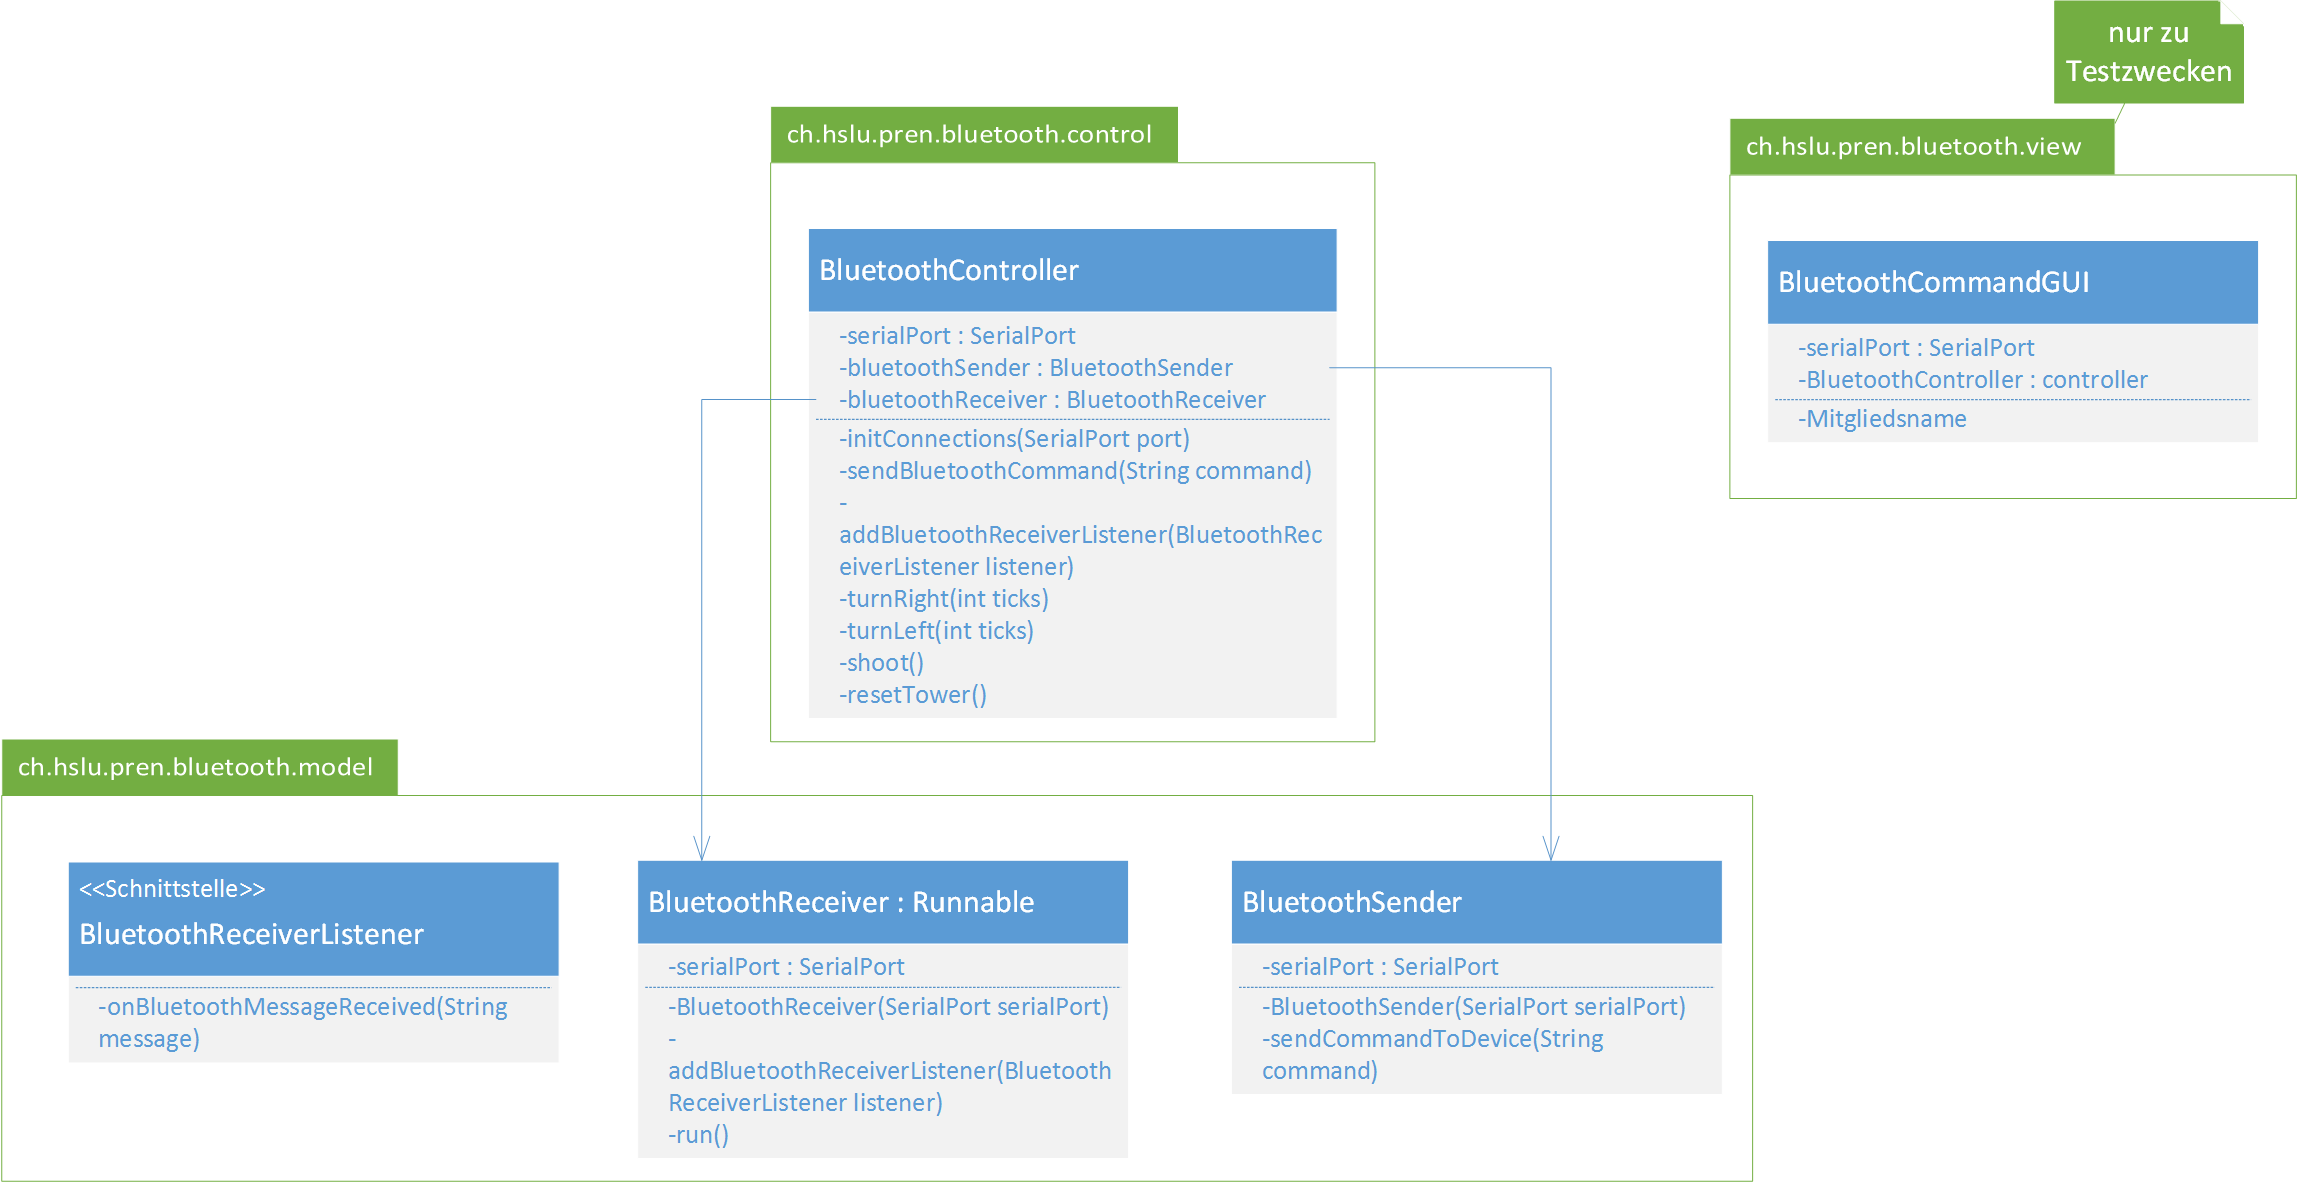
\includegraphics[width=1\textwidth]{../fig/Klassendiagramm Bluetoothmodul.png}
	\caption{Klassendiagramm Bluetoothmodul}
	\label{fig:Klassendiagramm Bluetoothmodul}        
\end{figure} \\
Details zu den Methoden und den verwendeten Datentypen sind in der JavaDoc festgehalten. \\
\paragraph{Einsatz, Abläufe, Voraussetzungen und Zusicherungen}
\begin{itemize}
	\item{Bevor Daten über die Schnittstelle ausgetauscht werden können, muss mittels 
\verb?initConnections(String serialPortName)? ein gültiger serieller Port definiert werden. Der konfigurierte Port gilt für alle darauf folgenden command-Aufrufe. }
	\item{Ein Wechsel des seriellen Ports, d.h. Umkonfigurierung mit \verb?initConnections(String serialPortName)?, ist nun jederzeit möglich.}
	\item{Eine Klasse, die das Interface \verb?BluetoothReceiverListener? implementiert, kann als Observer für empfangene Nachrichten des BluetoothReceivers fungieren.}
\end{itemize}
\paragraph{Aufbau und Konfiguration} 
Keine zusätzlichen Informationen. \\
\paragraph{Fehlerbehandlung}
Die Fehlerbehandlung wird über unchecked Exceptions realisiert. Details siehe JavaDoc. \\
\paragraph{Beispielverwendung}
Der folgende Codeausschnitt zeigt die Verwendung der Schnittstelle anhand einer beispielhaften Implementation BluetoothController: \\
\lstinputlisting[caption={Beispiel zur Verwendung des BluetoothControllers}]{../../sw/PrenManager/src/TestGUI/newClass.java}

\subsubsection{Spezifikation Bilderkennung}

\lstsettingjava

\begin{table}[h!]
	\begin{tabular}{|l|l|l|l|l|}
		\hline 
		Version & Datum & Autor & Bemerkung & Status \\ 
		\hline 
		1.0.0 & 26.03.2015 & SN & Initiale Fassung & freigegeben \\ 
		\hline 
		1.0.1 & 15.04.2015 & SN & Initiale Fassung & freigegeben \\ 
		\hline 
		2.0.1 & 07.05.2015 & PK & Anpassung für Erkennung-Klasse & freigegeben \\ 
		\hline 
	\end{tabular} 
	\caption{Steckbrief der Klasse Erkennung}
\end{table}

\paragraph{Operationen und Datenstukturen}

Die Schnittstelle stellt folgende Methoden und Datentypen zur Verfügung:  \\
\begin{figure}[h!]          
	\centering             
	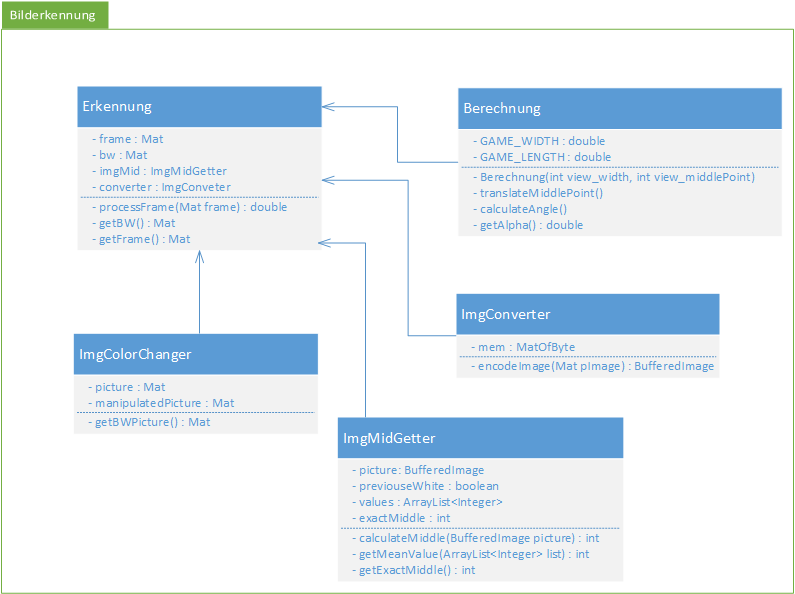
\includegraphics[width=0.5\textwidth]{fig/Klassendiagramm_Erkennung.png}
	\caption{Klassendiagramm Bilderkennung}
	\label{fig:Klassendiagramm Bilderkennung}        
\end{figure} \\
Details zu den Methoden und den verwendeten Datentypen sind in der JavaDoc festgehalten. \\

\paragraph{Einsatz, Abläufe, Voraussetzungen und Zusicherungen}
\begin{itemize}
	\item{Die Erkennung Klasse wird wie folgt initialisiert: \verb?Erkennung erkenner = new Erkennung();? }
	\item{Es gibt die Funktion \verb?processFrame(Mat frame)? mit welchem ein Bild abgearbeitet wird und den Winkel als double zurückliefert.}
\end{itemize}

\paragraph{Aufbau und Konfiguration} 
Keine zusätzlichen Informationen. \\

\paragraph{Fehlerbehandlung}
Die Fehlerbehandlung wird über unchecked Exceptions realisiert. Details siehe JavaDoc. \\

\paragraph{Beispielverwendung}
Der folgende Codeausschnitt zeigt die Verwendung der Schnittstelle anhand einer beispielhaften Implementation BluetoothController: \\
\lstinputlisting[caption={Beispiel zur Verwendung der Bilderkennung}]{../../sw/PrenManager/src/TestGUI/Erkennung-Example.java}

\subsubsection{Spezifikation ImageGetter}

\lstsettingjava

\begin{table}[h!]
	\begin{tabular}{|l|l|l|l|l|}
		\hline 
		Version & Datum & Autor & Bemerkung & Status \\ 
		\hline 
		1.0.0 & 30.03.2015 & KW & Initiale Fassung & freigegeben \\ 
		\hline 
		1.0.1 & 16.04.2015 & KW & Initiale Fassung & freigegeben \\ 
		\hline 
		2.0.1 & 14.05.2015 & KW & Anpassung Bilderkennung & freigegeben \\ 
		\hline 
	\end{tabular} 
	\caption{Steckbrief der Klasse ImageGetter}
\end{table}

\paragraph{Operationen und Datenstukturen}

Die Schnittstelle stellt folgende Methoden und Datentypen zur Verfügung:  \\
\begin{figure}[h!]          
	\centering             
	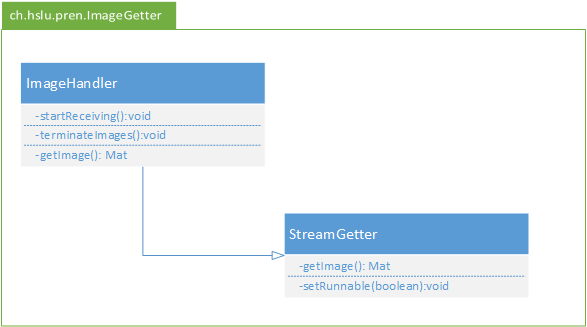
\includegraphics[width=0.5\textwidth]{../fig/Klassendiagramm_ImageGetter.png}
	\caption{Klassendiagramm ImageGetter}
	\label{fig:Klassendiagramm ImageGetter}        
\end{figure} \\
Details zu den Methoden und den verwendeten Datentypen sind in der JavaDoc festgehalten. \\

\paragraph{Einsatz, Abläufe, Voraussetzungen und Zusicherungen}
\begin{itemize}
	\item{Die ImageGetter-Klasse wird wie folgt initialisiert: \verb?ImageHandler imgHandler = new ImageHandler();? }
	\item{Mittels \verb?startReceiving()? der StreamGetter-Thread gestartet werden. Der StreamGetter steuert die Kamera an und speichert immer das aktuellste Bild. Dieses kann vom ImageHandler mittels \verb?getImage()? geholt werden. Der ImageHandler stellt dieses Bild dann mit der eigenen \verb?getImage()?-Funktion als Mat-Objekt zu Verfügung. Der Thread kann mittels \verb?terminateImages()? beendet werden.}
\end{itemize}

\paragraph{Aufbau und Konfiguration} 
Keine zusätzlichen Informationen. \\

\paragraph{Fehlerbehandlung}
Die Fehlerbehandlung wird über unchecked Exceptions realisiert. Details siehe JavaDoc. \\

\paragraph{Beispielverwendung}
Der folgende Codeausschnitt zeigt die Verwendung der Schnittstelle anhand einer beispielhaften Implementation ImageGetter: \\
\lstinputlisting[caption={Beispiel zur Verwendung des ImageGetters}]{../../sw/PrenManager/src/TestGUI/TestImageGetter.java}

\clearpage
\subsection{Softwaresubsysteme}
Nachfolgend sind die einzelnen Softwaresubsysteme und ihre Komponenten und Funktionalitäten beschrieben.
\subsubsection{Bluetoothmodul}
Das Bluetoothmodul setzt sich im Wesentlichen aus drei Komponenten zusammen. Diese Komponenten sind:
\begin{itemize}
	\item{\textbf{BluetoothSender:} Diese Klasse übernimmt die Befehlsübermittlung an das Freedomboard.}
	\item{\textbf{BluetoothReceiver:} Diese Klasse ist für das Empfangen der Statusnachrichten vom Freedomboard zuständig. Sie enthält eine Liste von BluetoothReceiverListener, deren Implementationen als Observer fungieren.}
	\item{\textbf{BluetoothController:} Der BluetoothController übernimmt die Initialisierung und Steuerung der einzelnen Komponenten und regelt deren Zusammenspiel. Er dient ausserdem als "'Durchlauferhitzer"' für BluetoothReceiverListener-Implementationen, damit diese sich beim BluetoothReceiver als Observer anmelden können.}
\end{itemize}

\subsubsection{Bilderkennung}
Um die Bilderkennung zu optimieren, wird statt des ganzen Bildes lediglich ein 
Teilausschnitt verwendet.  Der Bildausschnit wird mittels Maus-Drag 
ausgewählt. Der markierte Bereich wird danach auf dem Bildschirm dargestellt. \\

\noindent
Durch den kleineren Bildausschnitt, wird die Auswertung des Bildes schneller 
durchgeführt. Im folgenden sieht man wie der markierte Bereich auf dem 
Interface aussieht.\\

\begin{figure}[h!]          
	\centering             
	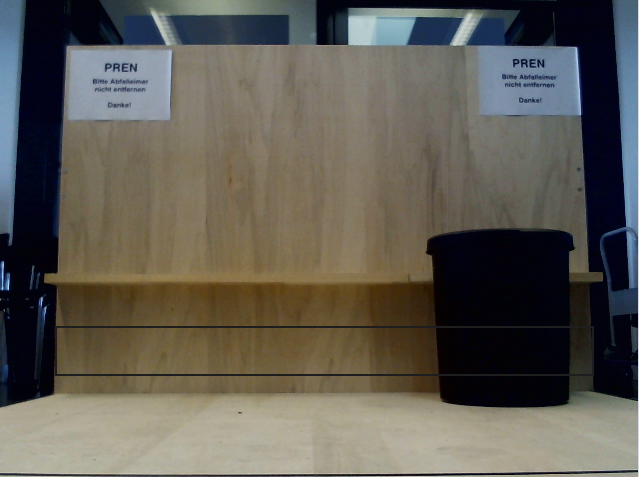
\includegraphics[width=1\textwidth]{fig/BildMitKorb_markiert.png}
	\caption{Bilderkennung - Ausschnitt}
	\label{fig:Bilderkennung_ausschnitt}        
\end{figure}

Der Ablauf der Bilderkennung funktioniert folgendermassen:
\begin{itemize}
	\item Der Bildausschnitt wird in ein schwarz/weiss Bild umgewandelt. \\
        Der Korb wird weiss, der Hintergrund schwarz dargestellt. 
	\item Ein Algorithmus scannt den Bildausschnitt Zeile für Zeile.
    \begin{itemize}
	    \item Es wird oben Links im Bildausschnitt gestartet.
	    \item Es wird Pixel für Pixel durchgelaufen und das erste weisse Pixel gespeichert.
	    \item Das Endpixel wird bestimmt, wenn auf das weisse Pixel ein schwazes Pixel folgt.
	    \item Von den Start und Endpunkte über die verschiedenen Zeilen wird der Mittelwert berechnet.
    \end{itemize}
\end{itemize}

\begin{figure}[h!]          
	\centering             
	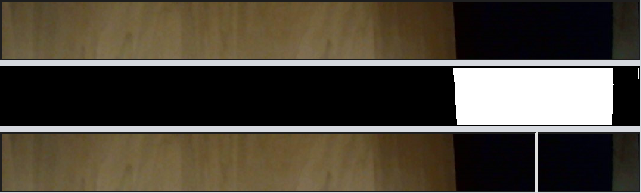
\includegraphics[width=1\textwidth]{fig/Korberkennung_Schritte.png}
	\caption{Bilderkennung - Ablauf}
	\label{fig:Bilderkennung_ablauf}        
\end{figure}

\noindent
Mit dem gefundenen Mittelwert kann anhand von Geometrie der Winkel von der 
Maschine zum Korb bestimmt werden.  Es tritt ein Problem bei der 
Winkelbestimmung auf, falls der Korb sich links oder rechts am Rand befindet.  
Da der Blick der Kamera kegelförmig ist, wird nicht der gesammte Korb erfasst. 
Die äussere Hälfte des Korbs fehlt und dies führt dazu, dass der Winkel zu 
klein ist. Das Problem wird behoben, indem bei der Überschreitung eines 
Maximalwertes, der Winkel um ca. ein Grad erhöht wird.

\clearpage
\section{Inbetriebnahme}
Hier werden die Inbetriebnahmetests beschrieben.

\subsection{Tests Einzelkomponenten}

Kurz nach der Endmontage werden die einzelnen Komponenten getestet. Eine erste Inbetriebnahme des Ballnachschubs zeigt, das die Funktion gewährleistet ist. Das Drehmoment des Servomotors genügt um die 5 Bälle nach oben zu befördern. Die Geschwindigkeit des Ballnachschubs kann mit der Betriebsspannung des Motors eingestellt werden, allerdings ist sie auf ca. 12V begrenzt, da anderenfalls der Motor überlastet wird.

Der BLDC Motor kann bereits angesteuert werden und über ein Netzgerät wird die Drehzahl eingestellt. Hier zeigt sich, dass der Pneu eine Unwucht hat. Leider kann diese Unwucht nicht mit konventionellen Massnahmen behoben werden, das es sich um Ungenauigkeiten in der Dicke und in der Form handelt. Mit der erforderten Drehzahl für die Schussweite von ca. 2m wirkt sich die Unwucht jedoch nicht auf die Konstruktion aus.

Mit dieser Konfiguration werden die ersten Ballwürfe gemacht. Zuerst wird der Ballnachschub sehr langsam eingestellt, so dass die Drehzahl des Motors nach einem Schuss wieder auch die Anfangsdrehzahl gestiegen ist. Da die Streuung der Reichweite ungewöhnlich stark variiert (ca. 0.5m), haben wir auf der Gegenseite des Rades ein Stück Gummi aufgeklebt, so dass die Reibung des Tennisballs grösser ist. So wird die Streuung auf ca. 0.2m verkleinert. 

\begin{figure}[h!]          
	\centering             
	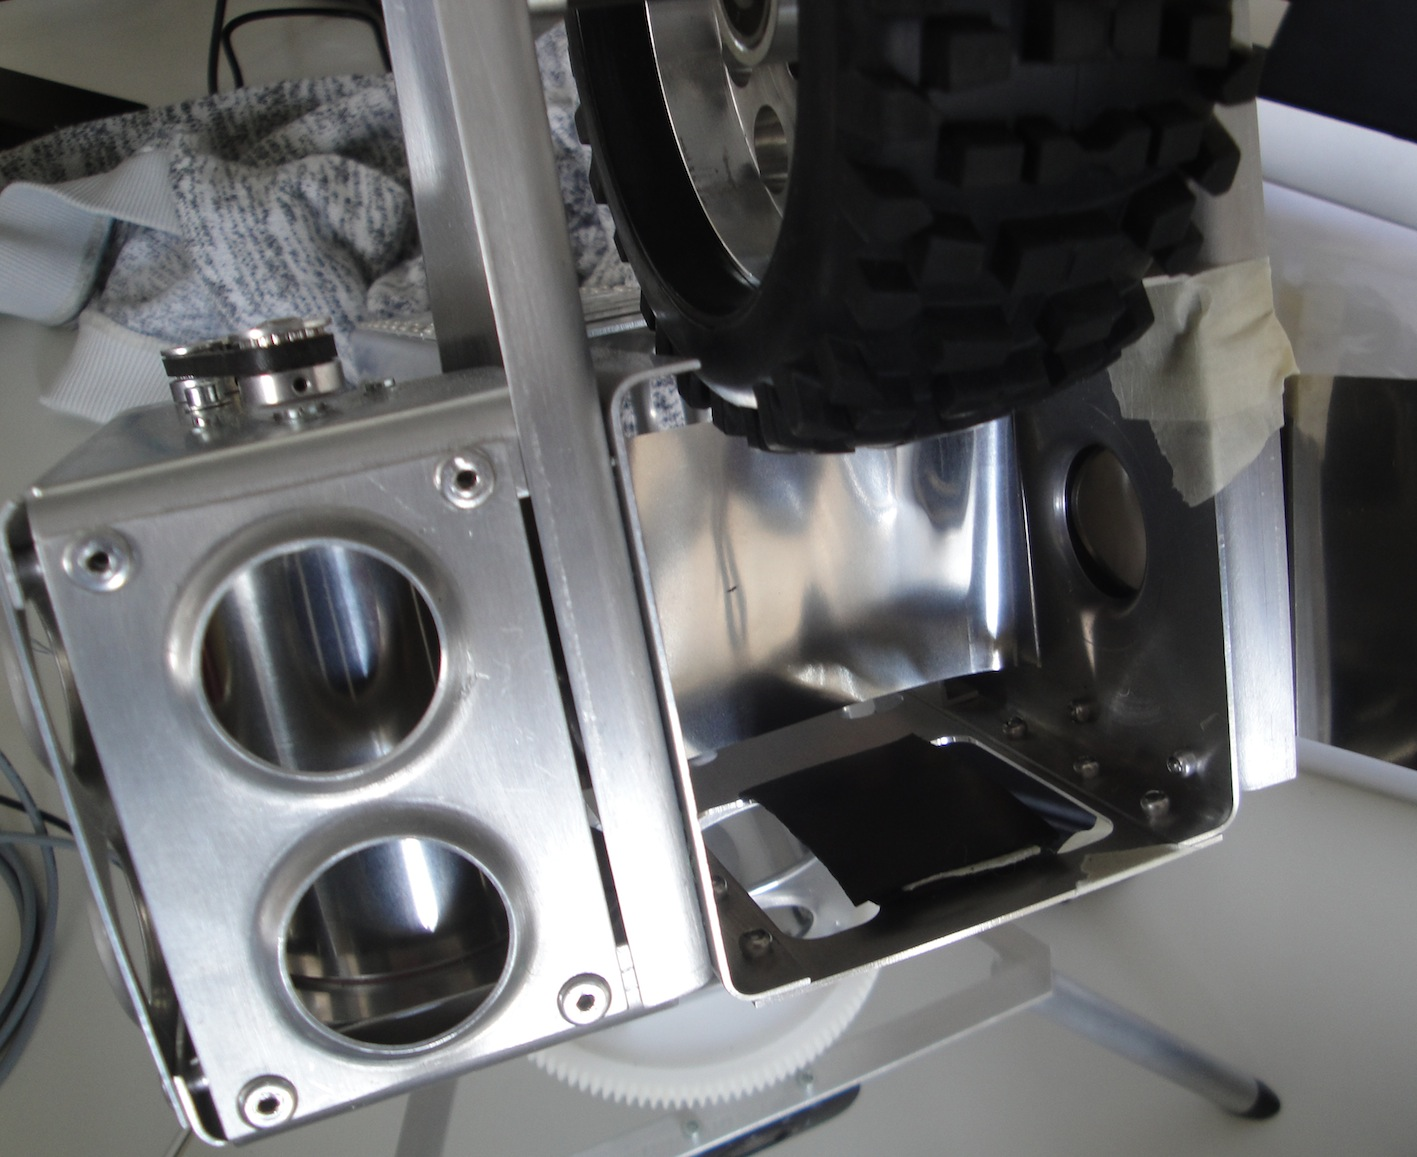
\includegraphics[width=0.5\textwidth]{fig/Bild_Gummi.JPG}
	\caption{Gummi zur Erhöhung der Reibung}
	\label{fig:Gummi}        
\end{figure}

In weiteren Tests werden die Bälle möglichst schnell nacheinander geschossen, so dass sich die Drehzahl des BLDC Motors nicht mehr ganz erholen kann. Komischerweise wird so die Streuung noch kleiner (nicht mehr von Auge abschätzbar). Drei weitere Tests mit Wettbewerbsbedingungen (Distanz und Höhe des Korbes) und mit schnellem Ballnachschub zeigen, dass die Genauigkeit sehr hoch ist, alle Bälle landen im Korb. Gegebenenfalls könnte mit einem anderen Pneu die Genauigkeit noch erhöht werden.

Die Drehvorrichtung funktioniert, und ist sehr schnell. Bei ersten Tests (ohne Tennisbälle) konnte innerhalb einer Sekunde mehr als eine Umdrehung gemacht werden. Schlussendlich muss sich der Turm nur um ca. 16$^\circ$ drehen, somit sollten ca. 1/5 Sekunde reichen um die Richtung einzustellen.



\subsection{Tests Gesamtsystem}
\subsubsection{Ablauf}
Die Tests des Gesamtsystems wurden durchgeführt, um das Zusammenspiel und richtige Funktionieren der einzelnen Komponenten zu gewährleisten. Dazu wird eine Bluetooth-Verbindung mit dem Gerät hergestellt. Da der BLDC-Motor beim Wettkampf bereits gestartet sein darf, wird dieser mittels Eingabefeld der Applikation bereits vor dem Wettkampfstart auf eine Drehzahl von \[\frac{1400\,Umdrehungen}{Minute}\] konfiguriert.

Anschliessend wird mittels Bilderkennung ein aktuelles Foto des Spielfelds geschossen. Auf diesem Foto wird per Mausziehen der Bereich des Spielfeldes ausgewählt. Wird nun das Startsignal gegeben, kann man einen Button drücken, der dann die Ausrichtung des Geräts übernimmt und den Ballnachschub nach einer Verzögerung von \[\frac{Anzahl\,Ticks}{20}\] in Bewegung setzt.

Sind alle Bälle geworfen worden, wird ein String an alle Observer des BluetoothReceivers gesendet. Enthält dieser String "fin", so heisst dies, dass das Gerät die Bälle alle verschossen hat und somit das Endsignal ausgelöst werden kann. Nach dem Endsignal ist der Test beendet.

\subsubsection{Resultate}

Die ersten Tests haben gezeigt, dass die Ballnachführung nicht zeitgleich mit dem Ausrichten in Bewegung gesetzt werden darf, da ansonsten der erste Ball nicht trifft. Integrationstests dieser beiden Komponenten haben gezeigt, dass die optimale Verzögerungszeit für den Start der Ballnachführung nach dem Ausrichten bei \[\frac{Anzahl\,Ticks}{20}\] liegt. 

Weitere Tests haben gezeigt, dass bei der Anfangs konfigurierten Drehzahl von 1372 pro Minute der erste Ball bei einem \[Ausrichtungswinkel > 16^\circ\] nicht trifft. Dies liegt daran, dass der erste Ball mit einer niedrigeren Geschwindigkeit an das Rad geführt wird, als die anderen Bälle. Dieses Problem ist nun behoben worden, indem der BLDC-Motor anfangs auf \[\frac{1400\,Umdrehungen}{Minute}\] eingestellt wird und zeitgleich zum Ausrichten auf \[\frac{1372\,Umdrehungen}{Minute}\] heruntergefahren wird. Tests mit dieser Konfiguration haben seither alle Bälle versenkt.overview
\clearpage
\section{Schlussdiskussion}
Wie bereits im Modul PREN1 stand für einen erfolgreichen Abschluss die 
Teamarbeit und ein gutes Zusammenspiel der unterschiedlichen Disziplinen im 
Vordergrund. Dem Team ist es gelungen trotz einiger Schwierigkeiten einen 
guten Weg zu finden um das geforderte Produkt zu fertigen. Hierbei konnte 
sowohl von den anderen Fachrichtungen sowie auch innerhalb der eigenen 
Disziplin neue Erfahrungen gesammelt werden. Die in der Gruppe herrschende 
Stimmung wurde als kollegial und lösungsorientiert empfunden. Diese 
Voraussetzungen ermöglichten optimale Arbeitsbedingungen und ein effektives 
Vorankommen.\\

\noindent
Das Produkt entspricht grösstenteils  dem in PREN1 ausgearbeitetem Entwurf. 
Durch frühzeitige Funktionstests und den damit verbundenen neuen Erkenntnissen 
während dem Zusammenbau, konnte das Produkt kontinuierlich verbessert werden 
und bietet so gegenüber dem ursprünglichen Entwurf einige Vorteile. Leider 
erforderten einige Funktionstests das Vorhandensein von Komponenten anderer 
Disziplinen, was teilweise zu Verzögerungen führte\\

\noindent
Einmal mehr zeigte sich, dass eine gute Planung des Projektablaufes und eine 
Strukturierung der noch bearbeiteten Aufgaben essenziell für das Gelingen 
eines Projektes sind. Durch ein regelmässiges Treffen der Gruppe und bei 
Bedarf einberufenen Sitzungen, bei welchen sämtliche Teammitglieder anwesend 
waren, konnte auch diese Schwierigkeit vorteilhaft bewältigt werden. Aufgrund 
von diesem reibungslosen Informationsaustausch konnten eigene Pendenzen und 
deren Relevanz für andere Teammitglieder eingeschätzt und die Planung 
verbessert werden.\\

\noindent
Abschliessend erhofft sich das Team 27 für den kommenden Wettbewerb ein gutes 
Gelingen und eine störungsfreie Ausführung der Aufgabe.\\

\clearpage
\listoffigures
\listoftables
%\nocite{*}
\renewcommand{\refname}{Literatur- und Quellenverzeichnis}
\bibliography{doc.bib}

\newcommand{\PRENETPATH}{cd}
%\newcommand{\PRENETPATH}{../../../../sem5/pren-et/doc}
\begin{appendix}
\clearpage
%\section{Sourcecode Steppertreiber L6480 von ST Microelectronics}
%\lstinputlisting[caption={l6480.c}]{../../../../sem5/pren-et/stepper/driver/drv/l6480.c}
%\lstinputlisting[caption={l6480.h}]{../../../../sem5/pren-et/stepper/driver/drv/l6480.h}
\clearpage
% Projektplanung
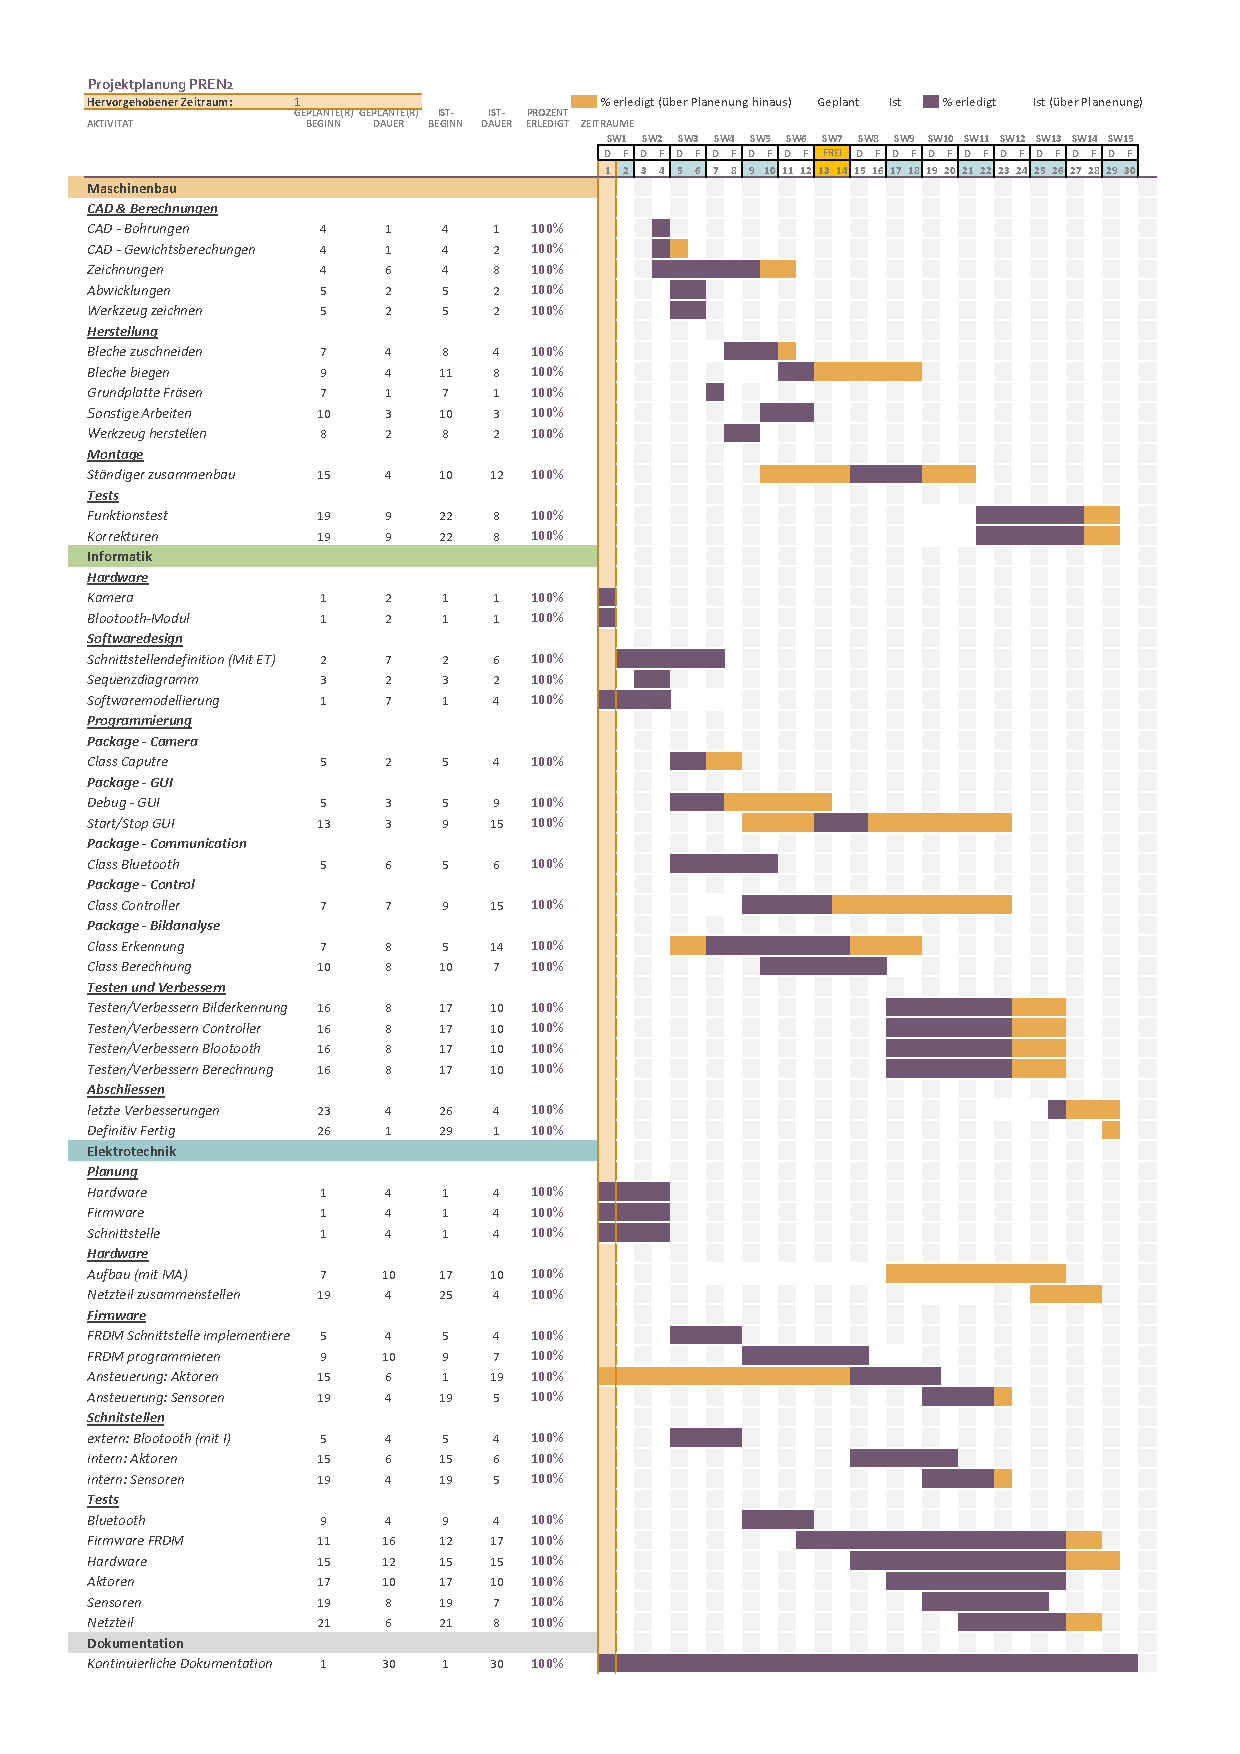
\includepdf[
    pages=1, 
    offset=0cm -2.5cm, 
    frame=false, 
    pagecommand={
        \textcolor{white}{\section{Anhang: Projektplanung}}
        \label{app:project}
        \thispagestyle{empty}}
    ]{cd/Projektplanung_DEF_11-06-2015v2.pdf}
% Drawings
\includepdf[
    pages=1, 
    offset=0cm -2.5cm, 
    frame=false, 
    angle=90,
    pagecommand={
        \textcolor{white}{\section{Anhang: Technische Zeichungen}}
        \label{app:drawing}
        \thispagestyle{empty}}
    ]{cd/Zeichnungen_komplett.pdf}
\includepdf[
    pages=2-, 
    offset=0cm -2.5cm, 
    frame=false, 
    angle=90,
    pagecommand={
        \thispagestyle{empty}}
    ]{cd/Zeichnungen_komplett.pdf}
% BLDC

\includepdf[
    pages=1, 
    offset=0cm -2.5cm, 
    frame=false, 
    pagecommand={
        \textcolor{white}{\section{Anhang: Dokumentation BLDC Motor Treiber}}
        \label{app:bldc}
        \thispagestyle{empty}}
    ]{\PRENETPATH/BLDC_StandaloneDoc.pdf}

\includepdf[
    pages=2-, 
    offset=0cm -2.5cm, 
    frame=false, 
    pagecommand={
        \thispagestyle{empty}}
    ]{\PRENETPATH/BLDC_StandaloneDoc.pdf}
% Stepper
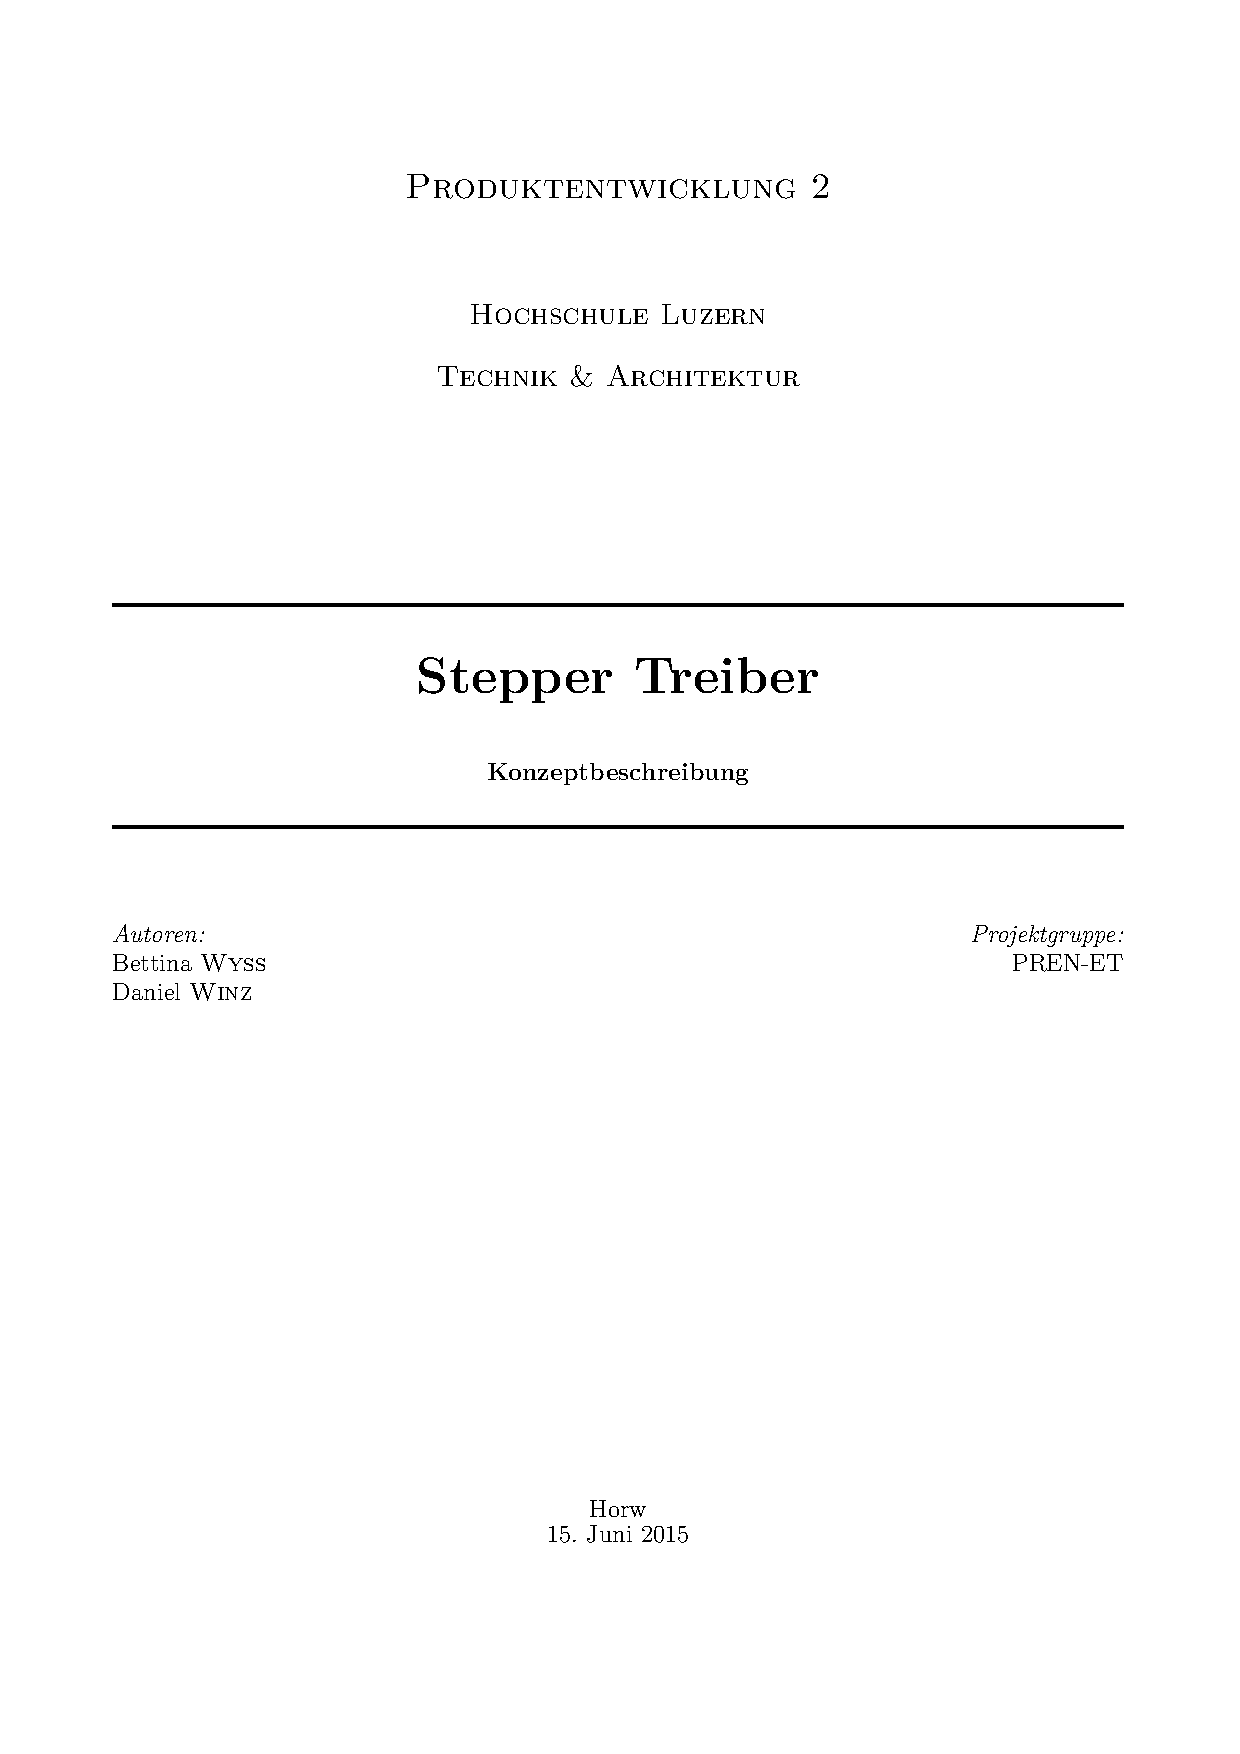
\includepdf[
    pages=1, 
    offset=0cm -2.5cm, 
    frame=false, 
    pagecommand={
        \textcolor{white}{\section{Anhang: Dokumentation Schrittmotor Treiber}}
        \label{app:stepper}
        \thispagestyle{empty}}
    ]{\PRENETPATH/Stepper_StandaloneDoc.pdf}
\includepdf[
    pages=2-, 
    offset=0cm -2.5cm, 
    frame=false, 
    pagecommand={
        \thispagestyle{empty}}
    ]{\PRENETPATH/Stepper_StandaloneDoc.pdf}
% DC

\includepdf[
    pages=1, 
    offset=0cm -2.5cm, 
    frame=false, 
    pagecommand={
        \textcolor{white}{\section{Anhang: Dokumentation DC Motor Treiber}}
        \label{app:dc}
        \thispagestyle{empty}}
    ]{\PRENETPATH/DC_StandaloneDoc.pdf}

\includepdf[
    pages=2-, 
    offset=0cm -2.5cm, 
    frame=false, 
    pagecommand={
        \thispagestyle{empty}}
    ]{\PRENETPATH/DC_StandaloneDoc.pdf}
% Review PREN-ET
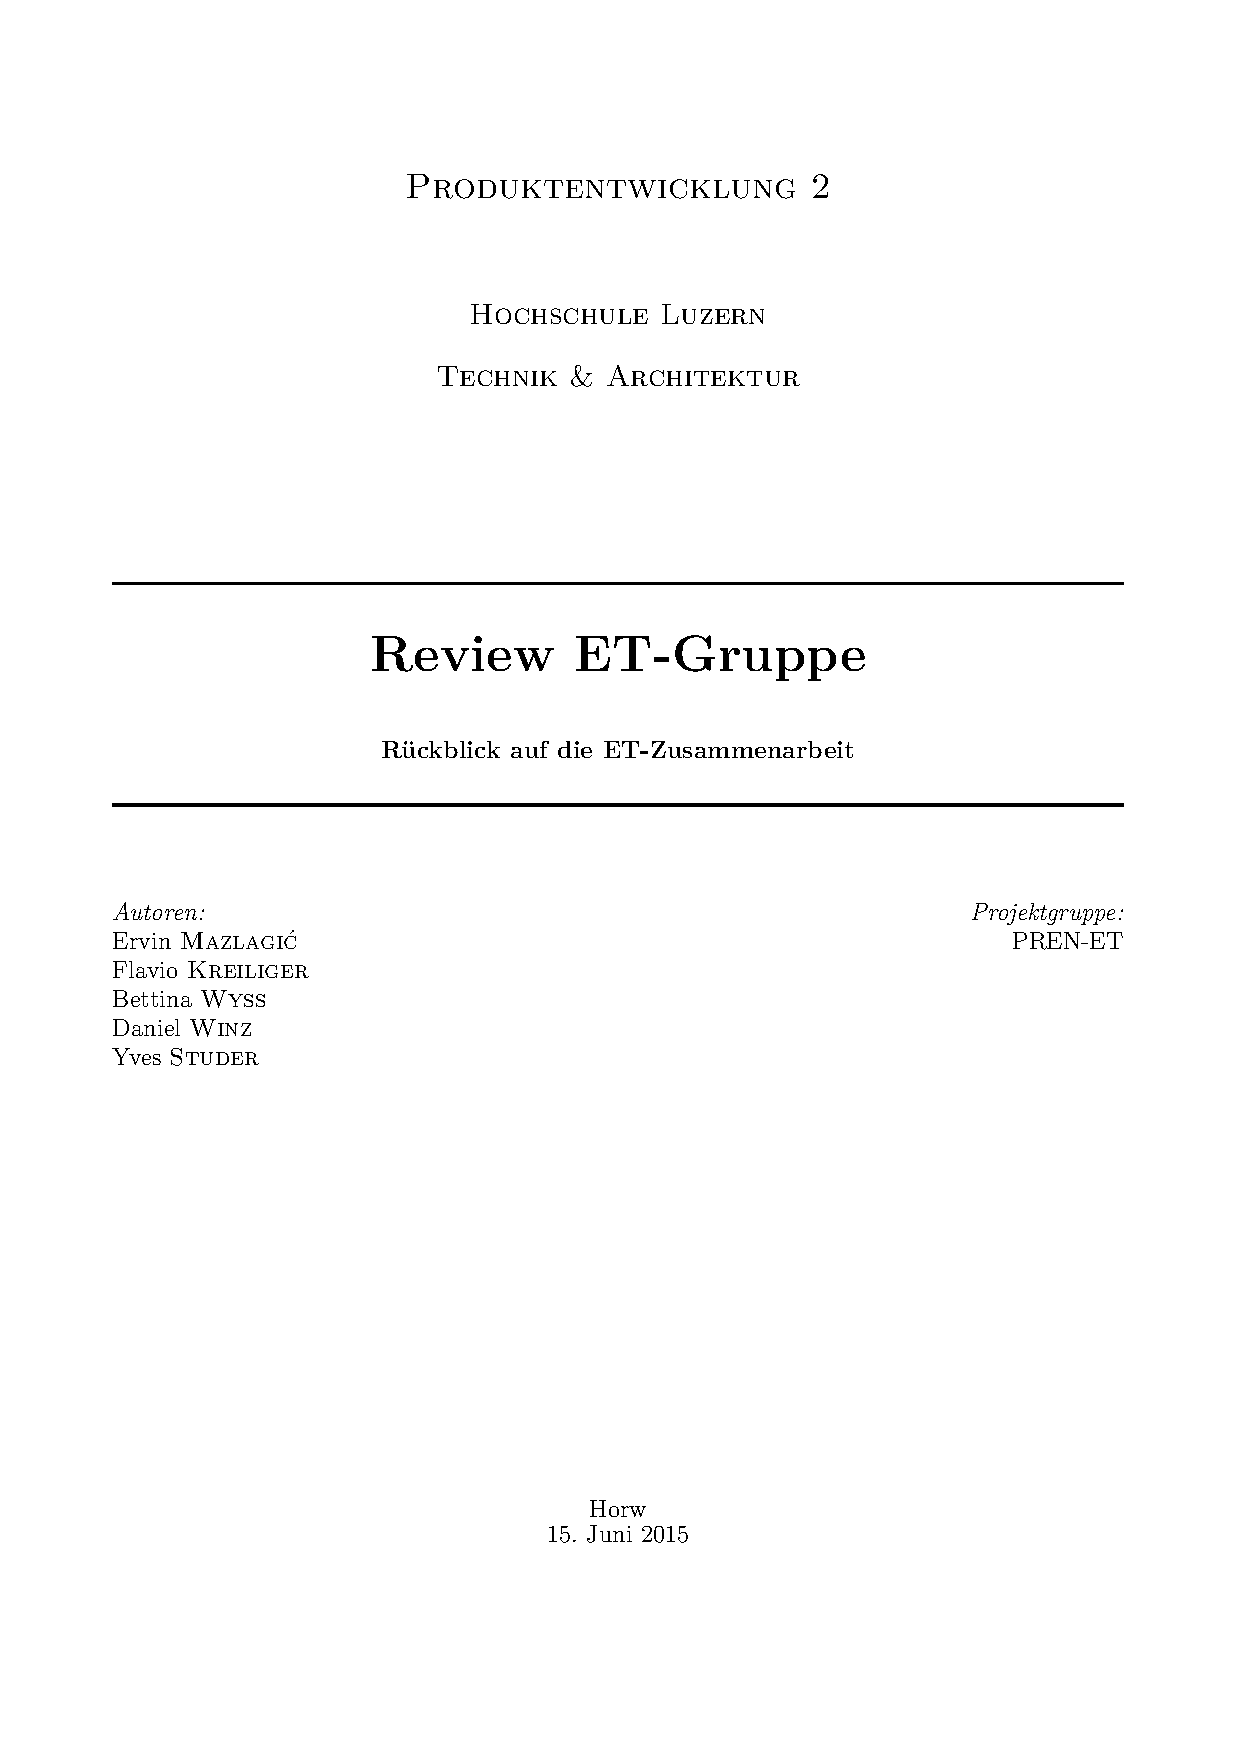
\includepdf[
    pages=1, 
    offset=0cm -2.5cm, 
    frame=false, 
    pagecommand={
        \textcolor{white}{\section{Anhang: Review PREN-ET}}
        \label{app:dc}
        \thispagestyle{empty}}
    ]{\PRENETPATH/ET-Gruppe_Review.pdf}
\includepdf[
    pages=2-, 
    offset=0cm -2.5cm, 
    frame=false, 
    pagecommand={
        \thispagestyle{empty}}
    ]{\PRENETPATH/ET-Gruppe_Review.pdf}
% Aufgabenstellung
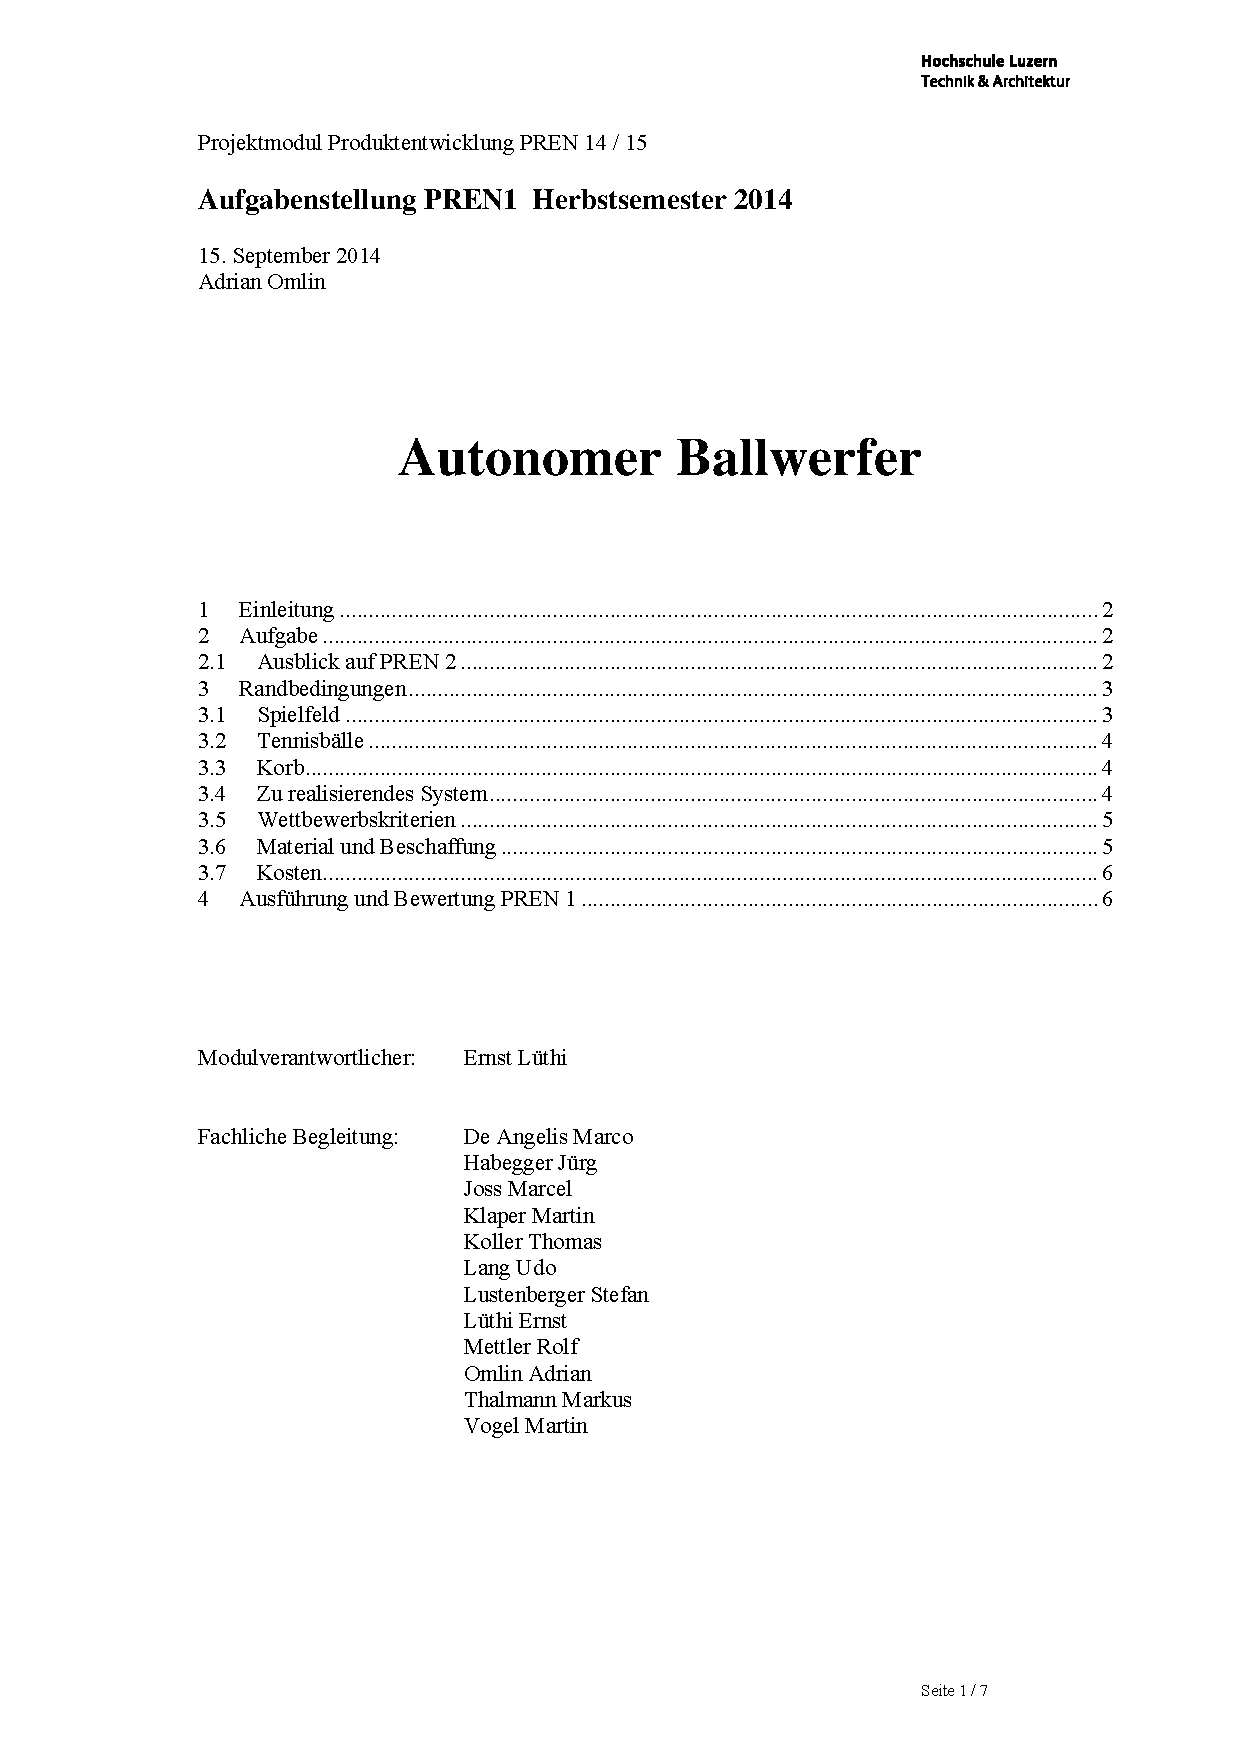
\includepdf[
    pages=1, 
    offset=0cm -2.5cm, 
    frame=false, 
    pagecommand={
        \textcolor{white}{\section{Anhang: Aufgabenstellung}}
        \label{app:aufgabe}
        \thispagestyle{empty}}
    ]{cd/Aufgabenstellung_PREN1_H14.pdf}
\includepdf[
    pages=2-, 
    offset=0cm -2.5cm, 
    frame=false, 
    pagecommand={
        \thispagestyle{empty}}
    ]{cd/Aufgabenstellung_PREN1_H14.pdf}
\end{appendix}

